% !TeX program = lualatex
% !BIB program = biber
% !TeX encoding = UTF-8
% !TeX spellcheck = en_US
\documentclass[a4paper,12pt]{article}

% titlepage/metadata definitions
\newcommand{\thetitle}{High Performance Computing with Python}
\newcommand{\thesubtitle}{-- Final Report --}
\newcommand{\theauthor}{Peter Würth}
\newcommand{\thematnr}{5306261}
\newcommand{\theemail}{peter.wuerth@students.uni-freiburg.de}
\newcommand{\thedate}{\today}

% LTeX: enabled=false

% language
\usepackage[english]{babel}

% font
\usepackage[T1]{fontenc}
\usepackage{lmodern}
\renewcommand{\familydefault}{\sfdefault}

% spacing
\usepackage[onehalfspacing]{setspace}
% \usepackage[textwidth=15cm, textheight=22cm]{geometry}
\usepackage{enumitem}
\setlist{noitemsep}

% bibliography
\usepackage[backend=biber, sorting=none]{biblatex}
\addbibresource{literature.bib}
\DefineBibliographyStrings{english}{
    url={[Online]\adddot\addspace URL}
}
% FIX: warning: Font shape `T1/lmss/m/sc' in size <12> not available (Font)	Font shape `T1/lmr/m/sc' tried instead.
% -> lmodern does not have a small caps (sc) font
\renewcommand{\mkbibacro}[1]{{\footnotesize\MakeUppercase{#1}}}

% media
\usepackage{graphicx}
\graphicspath{{media/}}
\usepackage{subcaption}
\usepackage[font=small, labelfont=bf]{caption}
\usepackage[x11names]{xcolor}
\usepackage{tikz}
\usetikzlibrary{arrows.meta}
\usetikzlibrary{calc}
\usetikzlibrary{fit}
\usetikzlibrary{math}
\usetikzlibrary{positioning}
\usetikzlibrary{shapes.arrows}

% math
\usepackage{amsmath}
\usepackage{amsfonts}

% code snippets
\usepackage[outputdir=out, cachedir=_minted/cache]{minted}
\newminted{py}{ % environment: pycode
    autogobble,
    fontsize=\fontsize{8.5pt}{11pt},
    frame=single,
    framesep=8pt,
    mathescape,
    escapeinside=!!,
    texcomments
}
\newmintinline{py}{} % command: pyinline

% quoting
\usepackage{csquotes}

% links
\usepackage[pdfencoding=auto]{hyperref}
\hypersetup{
    pdftitle={\thetitle},
    pdfauthor={\theauthor},
    pdfcreator={LuaLaTeX},
    breaklinks,
    hidelinks,
    bookmarksnumbered=true,
    pageanchor=true,
}
\usepackage[capitalize, nameinlink, noabbrev]{cleveref}

% glossaries
\usepackage[nowarn]{glossaries}
\glsdisablehyper % since there is no \makeglossaries

\usepackage{fancyhdr}

\begin{document}

    % title page
    \begin{titlepage}
        \begin{center}
            \begin{singlespace}
                
\includegraphics[width=0.5\linewidth]{logo-uni-freiburg.eps}\\[4\baselineskip]
                {\huge\textbf{\thetitle}}\\[1\baselineskip]
                {\Large\thesubtitle}\\[3\baselineskip]
                {\large \theauthor \\ \thematnr \\ \theemail}\\\vfill
                \thedate
            \end{singlespace}
        \end{center}
    \end{titlepage}

    % table of contents
    \pagenumbering{gobble}
    \pdfbookmark{Contents}{toc}
    \tableofcontents

    % main content
    \pagenumbering{arabic}
    \section{Introduction}

    \section{Lattice Boltzmann Method}

    \section{Implementation}

    \section{Experiments}

This chapter presents the results obtained from various experiments performed with the implementation introduced in the previous chapter in order to validate the correctness of the implementation and test it's scaling behavior.

\subsection{Shear Wave Decay}

Shear wave decay describes the time evolution of a velocity or density perturbation, which converges to zero due to the effects of viscosity. In order to have a known analytical solution to compare the simulation results against, the experiments use sinusoidal perturbation as initial conditions and observes how they evolve over time. These initial perturbation are given in \cref{eq:swd:init-density,eq:swd:init-velocity} for an experiment with a density or velocity perturbation respectively. The initial density is given by $\rho_0$ and $\varepsilon$ defines the amplitude of the sine and therefore the max. perturbation.
\begin{subequations}
    \begin{equation}
        \rho(x, t=0) = \rho_0 + \varepsilon~\text{sin}\left(\frac{2 \pi x}{L_x}\right)
        \label{eq:swd:init-density}
    \end{equation}
    \begin{equation}
        u_x(x, t=0) = \varepsilon~\text{sin}\left(\frac{2 \pi x}{L_y}\right)
        \label{eq:swd:init-velocity}
    \end{equation}
\end{subequations}

The analytical solution is given by the Navier-Stokes equations for incompressible fluids:
\begin{equation}
    \frac{\partial u}{\partial t} + (u\cdot\nabla)u + \frac{1}{\rho}\nabla p = \nu\nabla^2u
    \label{eq:swd:navier-stokes}
\end{equation}
Since there is no analytical solution, we make two assumptions:
\begin{enumerate}
    \item the perturbation is small, therefore the velocity gradient is small enough to neglect the non-linear term $(u\cdot\nabla)u$
    \item the pressure gradient $\nabla p$ is small and negligible
\end{enumerate}
This yields then following analytical solution:
\begin{equation}
    a(t) = a_0 + \varepsilon~\text{exp}\left(-\nu \left(\frac{2\pi}{L}\right)^2 t\right)
    \label{eq:swd:analytica-solution}
\end{equation}

It describes a decaying exponential governed by the viscosity $\nu$ and the initial perturbation $\varepsilon$. The additional offset $a_0$ corresponds to $\rho_0$ in case of a sinusoidal density perturbation and is $0$ for the sinusoidal velocity perturbation. \cref{fig:swd:sines,fig:swd:density:decay,fig:swd:velocity:multiple-omega} show how the perturbation for both the sinusoidal density and velocity evolve over time and how the compare to the analytical solution given by \cref{eq:swd:analytica-solution}.

\begin{figure}[ht!]
    \begin{subfigure}{0.514\linewidth}
        \centering
        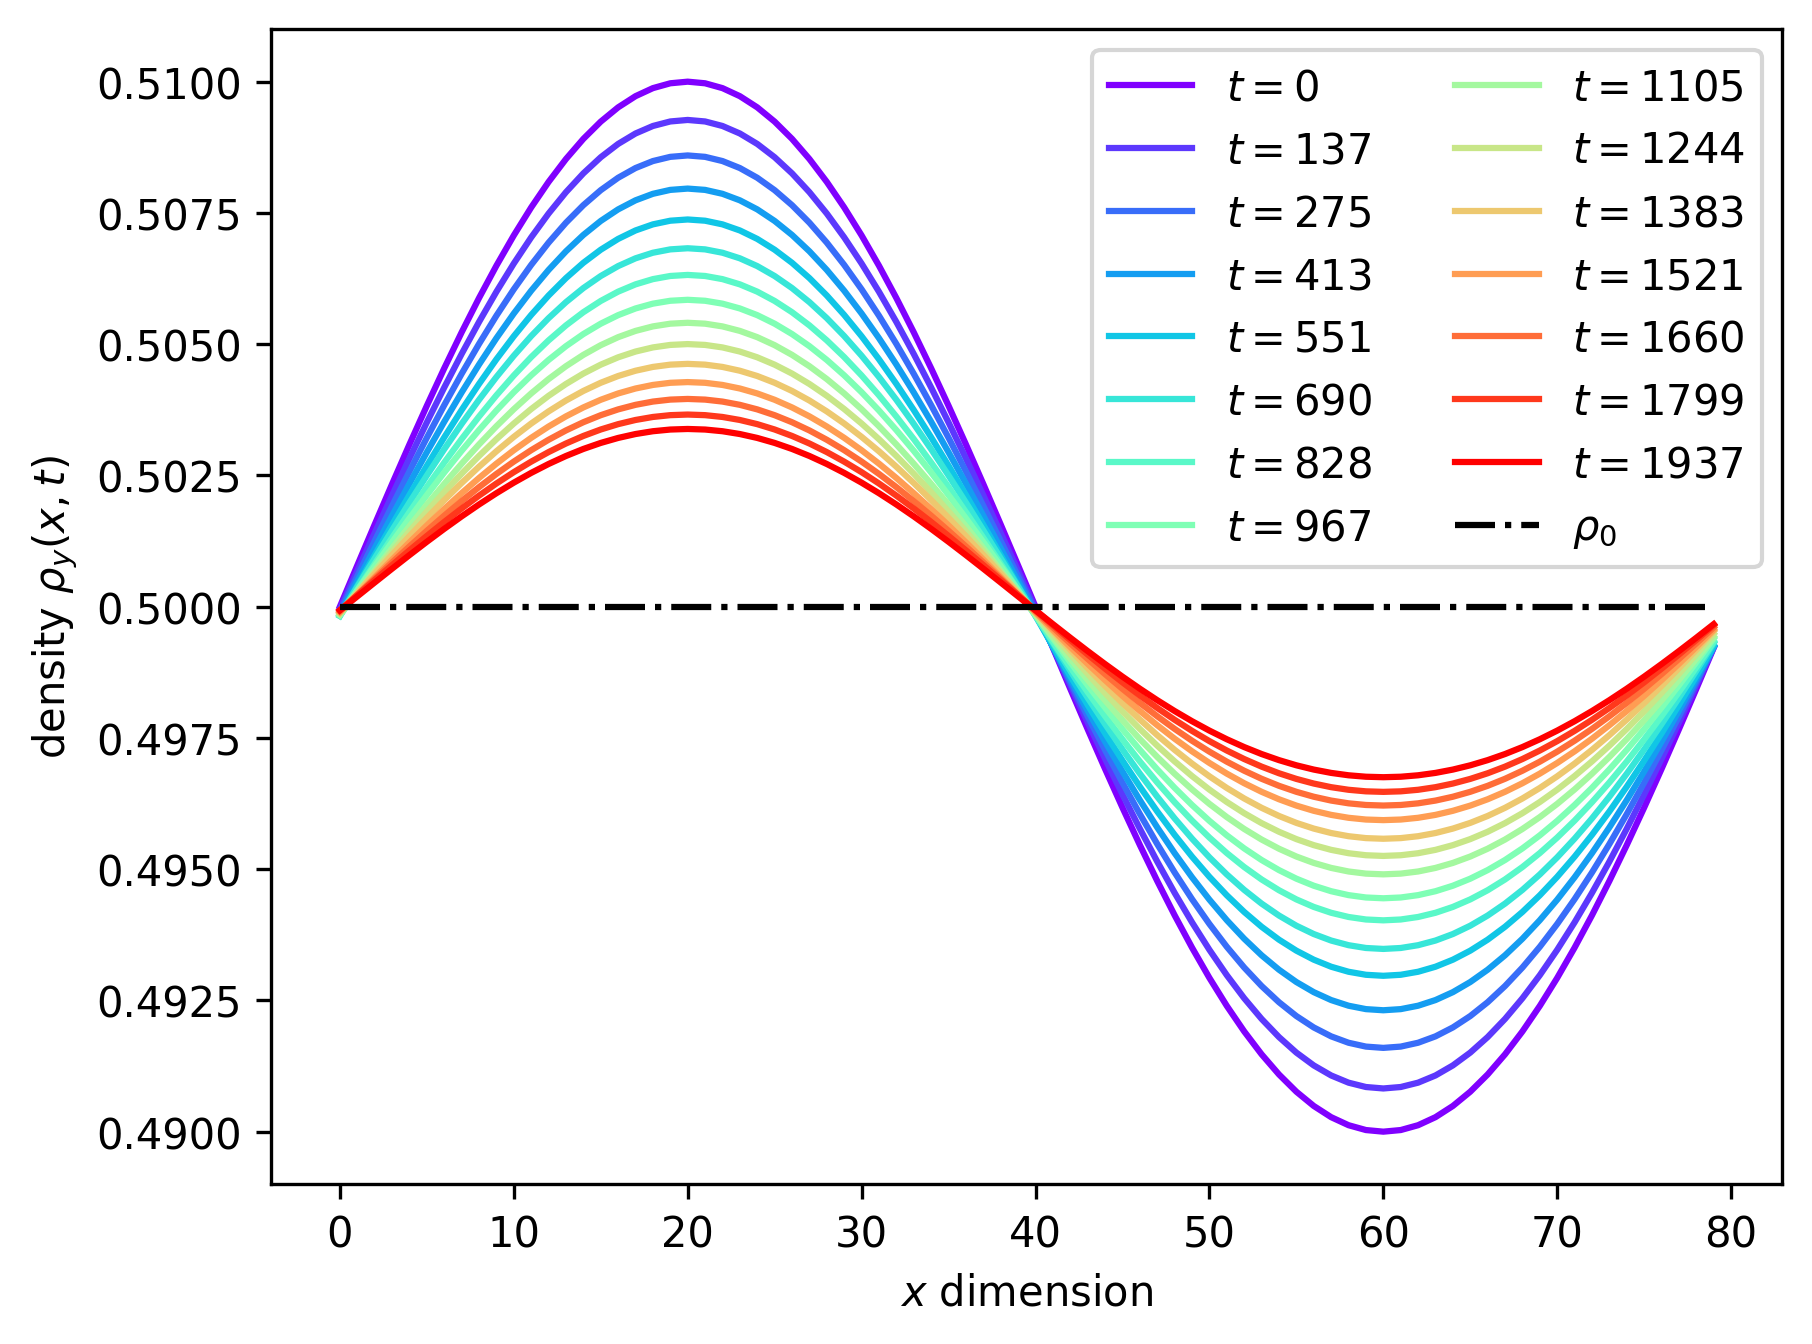
\includegraphics[width=\linewidth]{m3_density_decay_sine_evolution.png}
        \caption{Sinusoidal density}
        \label{fig:swd:density:sine}
    \end{subfigure}%
    \begin{subfigure}{0.486\linewidth}
        \centering
        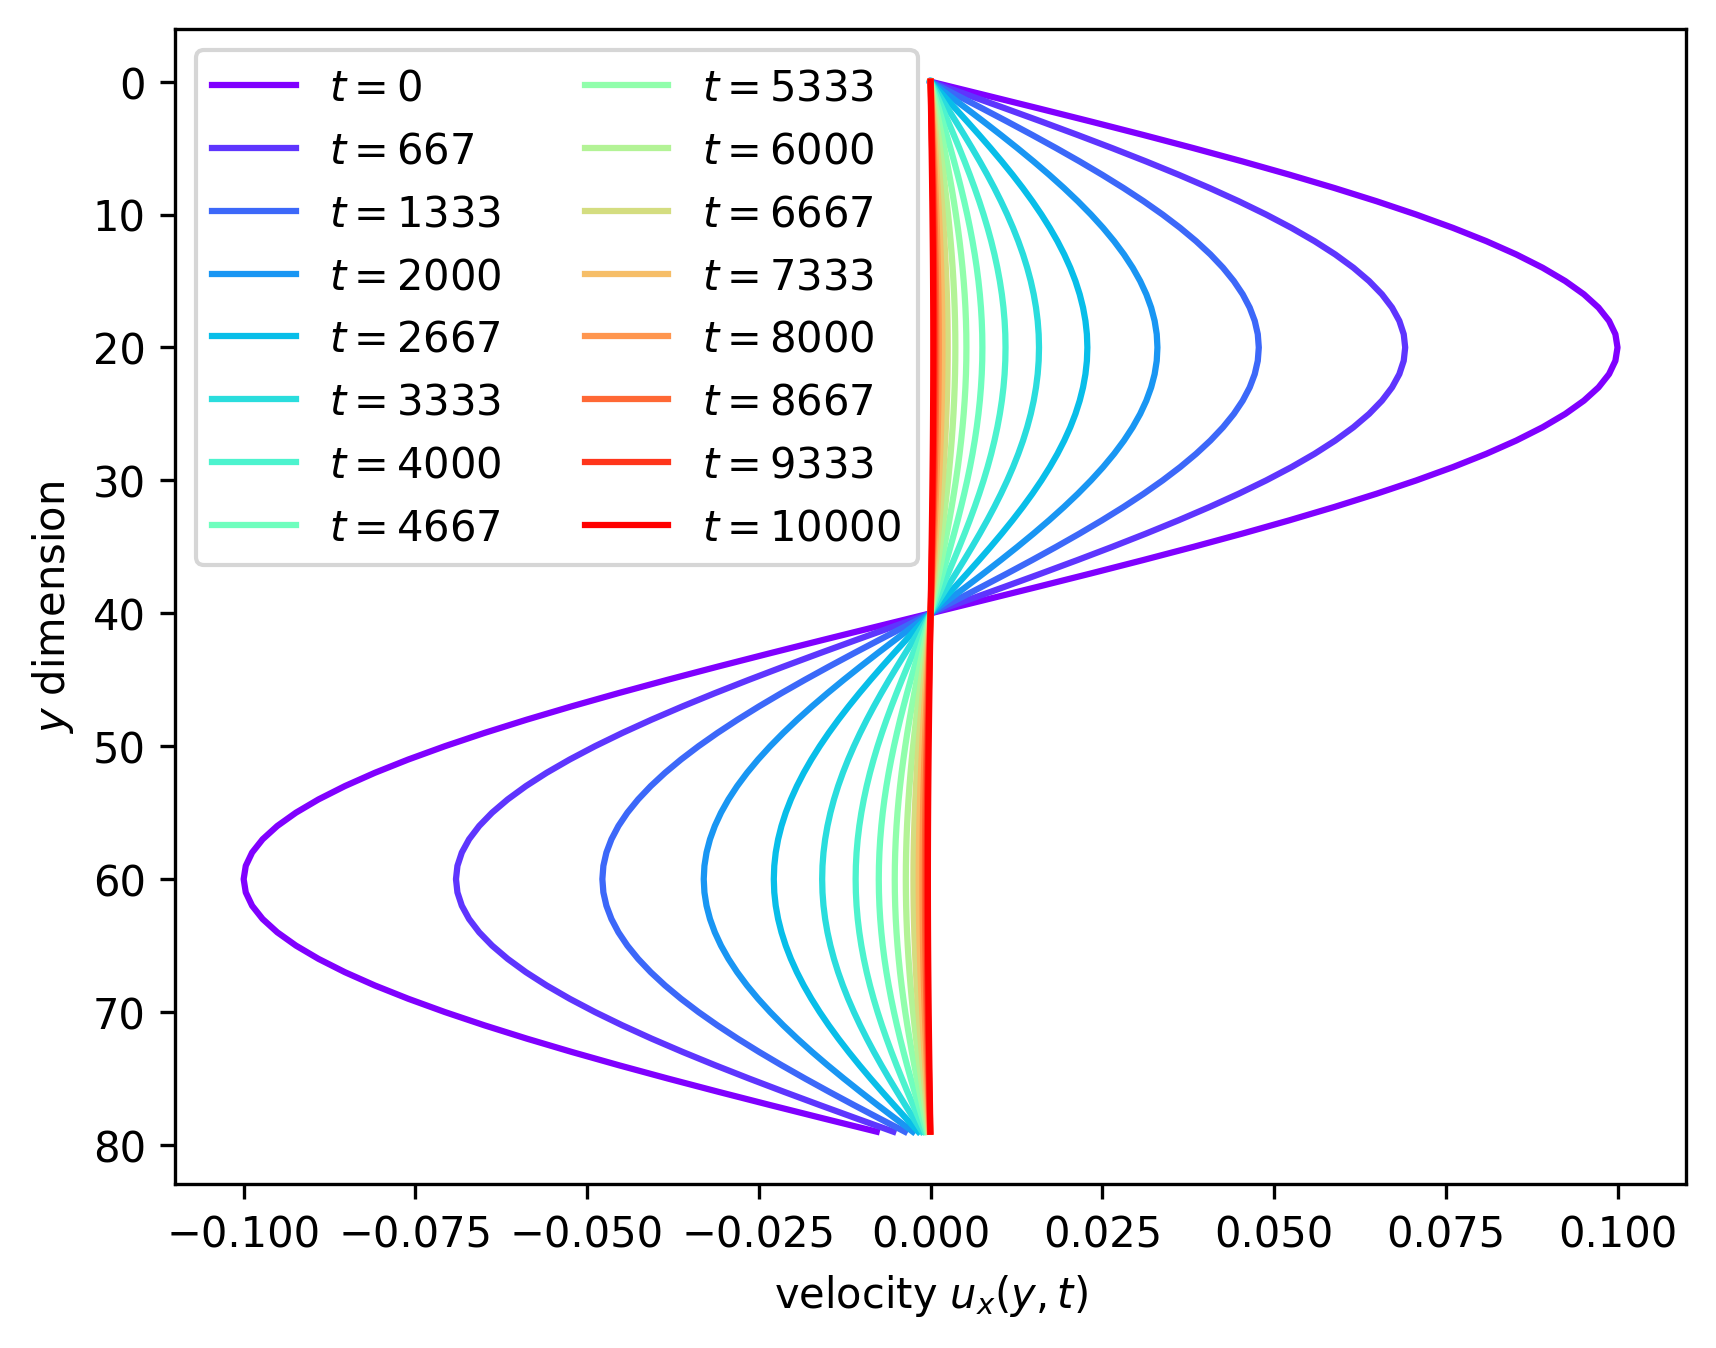
\includegraphics[width=\linewidth]{m3_velocity_sine_evolution.png}
        \caption{Sinusoidal velocity}
        \label{fig:swd:velocity:sine}
    \end{subfigure}
    \caption[Shear Wave Decay: Evolution of the perturbation sine wave]{Shear Wave Decay: Evolution of the perturbation sine wave. The parameters for (a) and (b) are the same as in \cref{fig:swd:density:multiple-omega,fig:swd:velocity:multiple-omega} respectively for $\omega=1.3$.}
    \label{fig:swd:sines}
\end{figure}

As expected, the perturbations retain their sinusoidal shapes but lose amplitude over time, compare \cref{fig:swd:sines}. While for the velocity decay the sinusoidal perturbation is stationary in position, the sinusoidal density decay is not, since high-density areas constantly flowing into low-density areas while converging to the equilibrium state. Therefore, observing the density at a fixed $x$-position results in an oscillating decay where only the peaks align with the analytical solution as depicted in \cref{fig:swd:density:single-omega}. The velocity decay on the other hand completely aligns with the analytical solution as seen in \cref{fig:swd:velocity:multiple-omega}.

\begin{figure}[ht!]
    \begin{subfigure}{\linewidth}
        \centering
        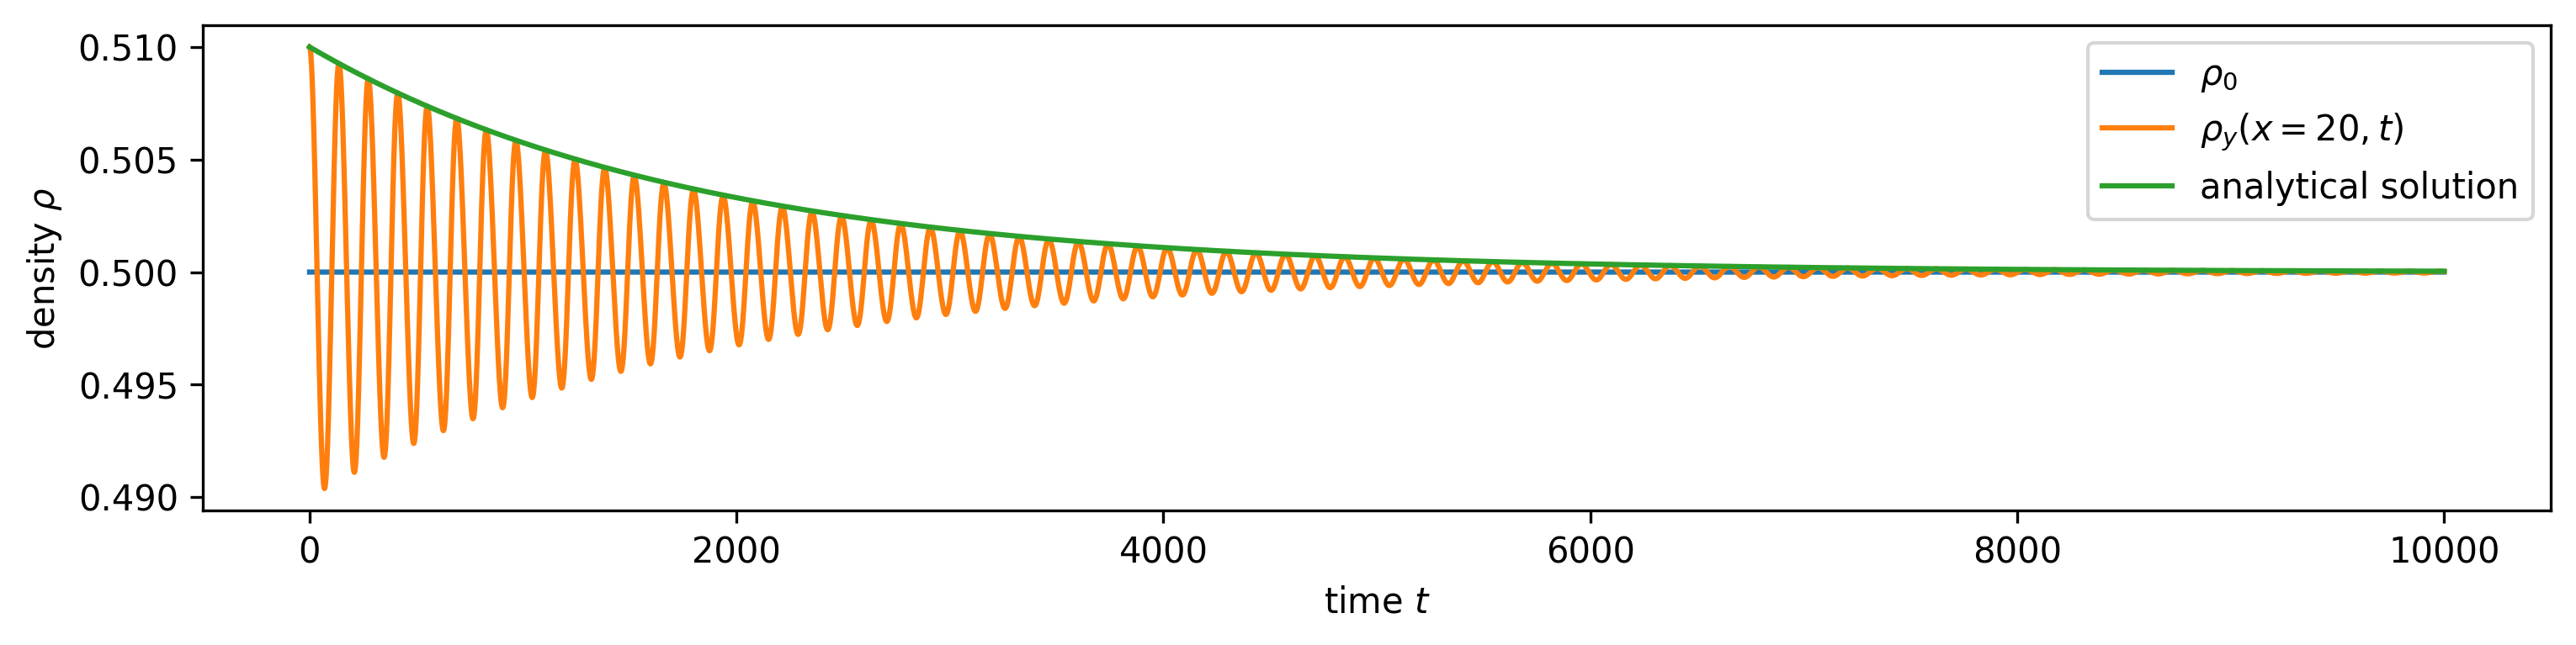
\includegraphics[width=\linewidth]{m3_density_decay_single_omega.png}
        \caption{Oscillating decay, $\omega=1.3$}
        \label{fig:swd:density:single-omega}
    \end{subfigure}

    \begin{subfigure}{\linewidth}
        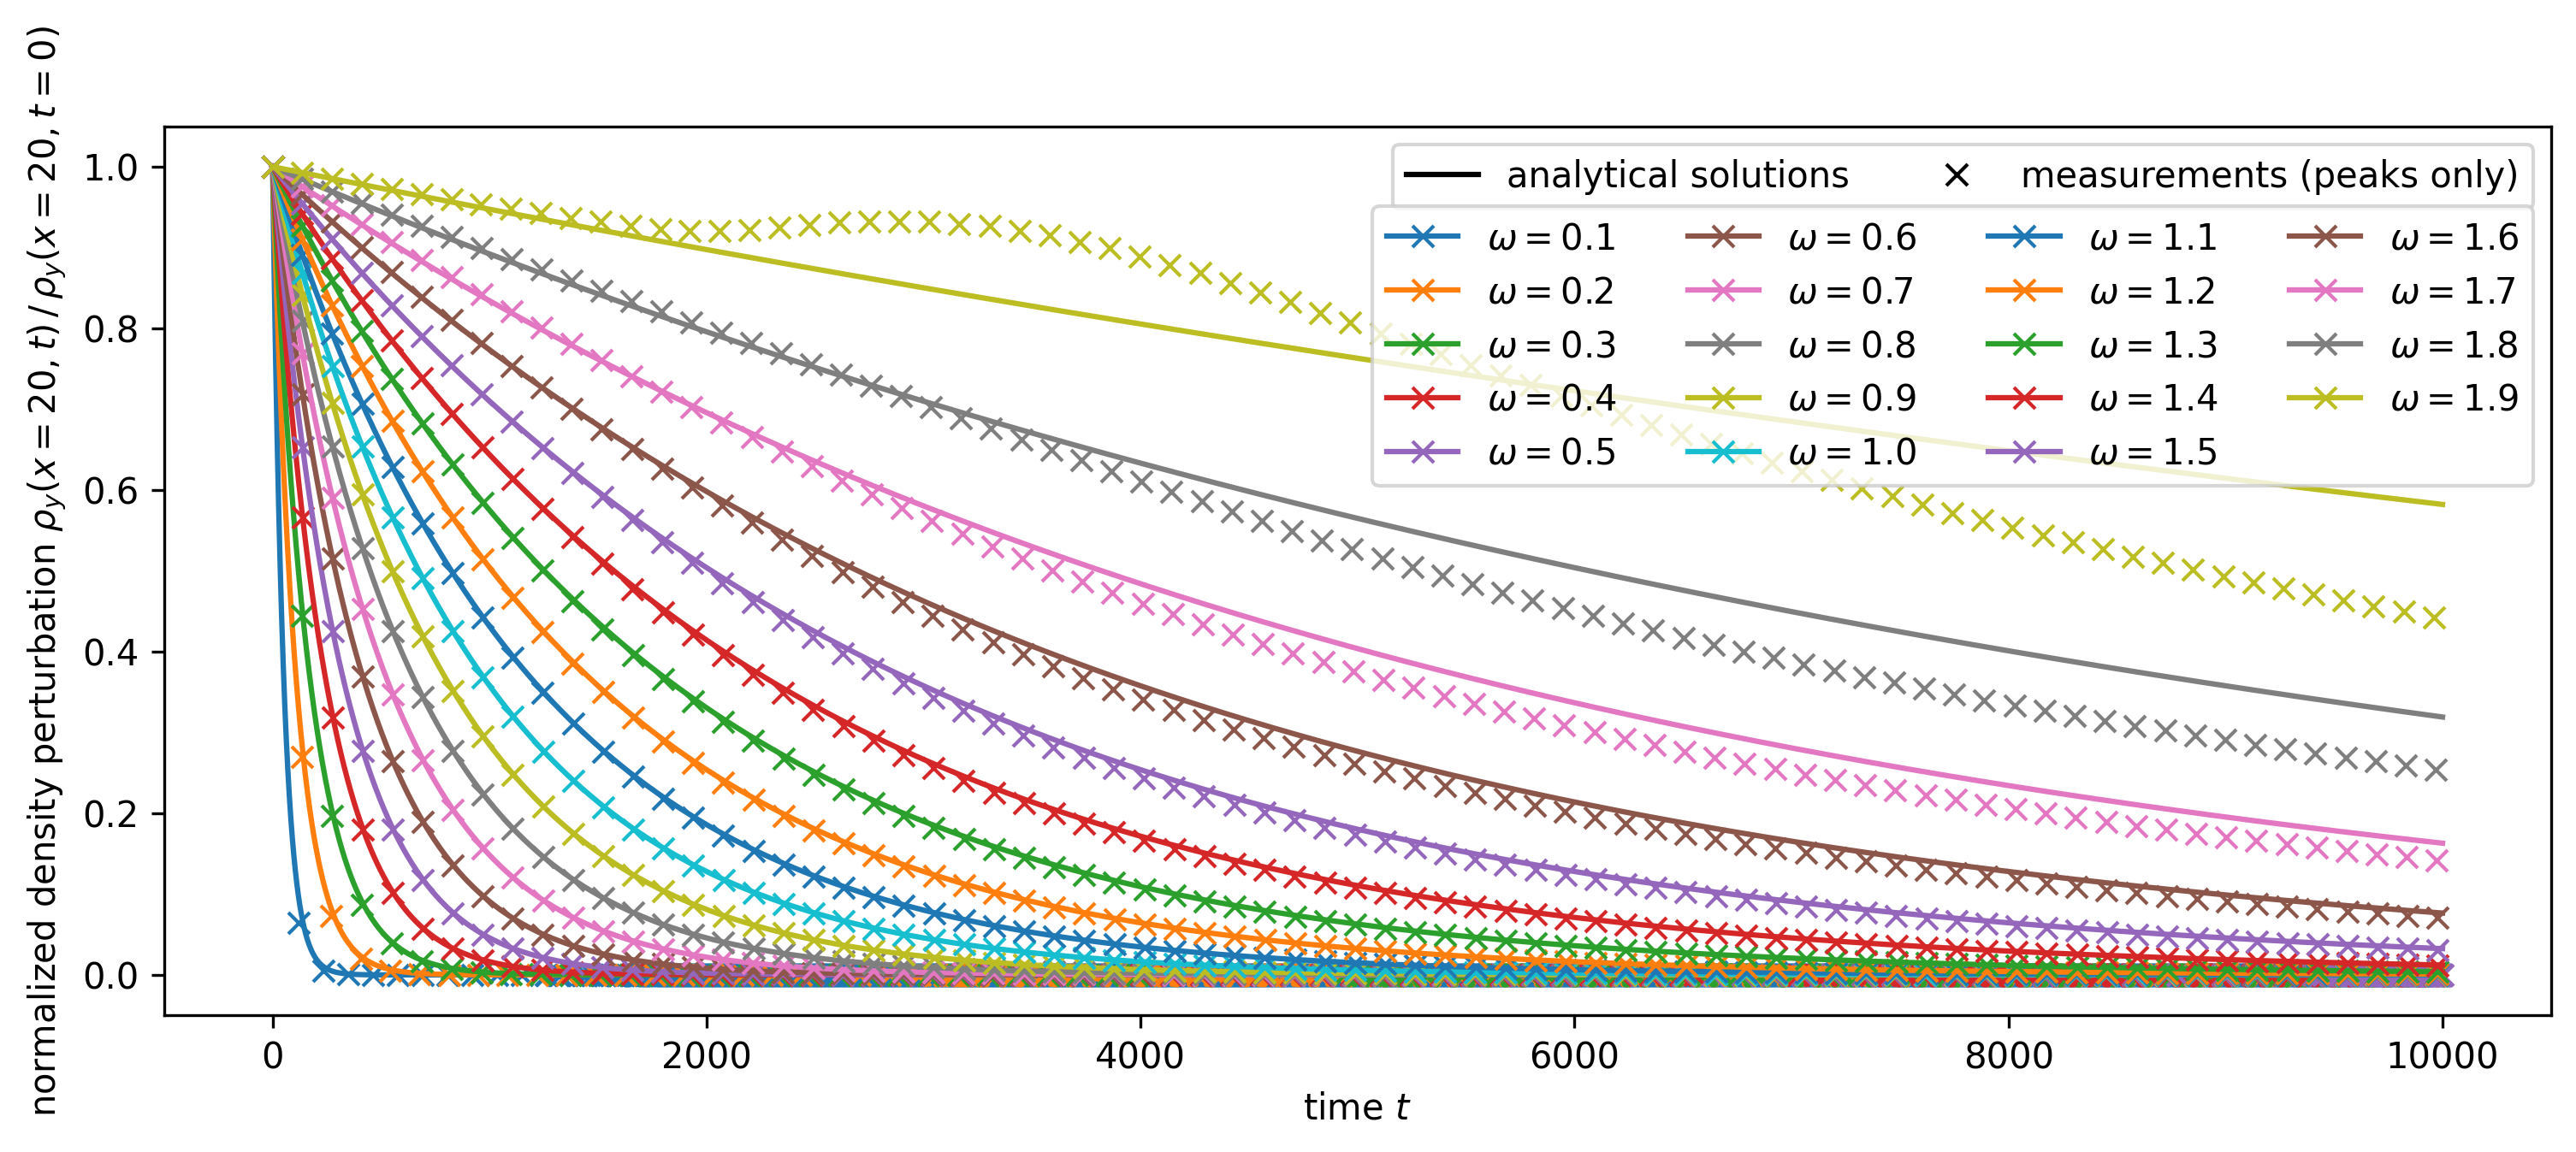
\includegraphics[width=\linewidth]{m3_density_decay_different_omegas_normalized.png}
        \caption{Peaks only, multiple $\omega$}
        \label{fig:swd:density:multiple-omega}
    \end{subfigure}

    \caption[Shear Wave Decay: Normalized time evolution of the sinusoidal density decay for different relaxation rates $\omega$]{Shear Wave Decay: Normalized time evolution of the sinusoidal density decay for different relaxation rates $\omega$. The measured values are given by the oscillating, sinusoidal density at $x=20$ for a lattice of size $80\times20$. They are set in relation to the analytical solution given by \cref{eq:swd:analytica-solution}. While (a) shows the complete oscillating decay, (b) only shows the peaks for the sake of better depiction. The simulation was run for $10000$ steps and with the coefficients $\rho_0=0.5$ and $\varepsilon=0.01$ for the initial sinusoidal density as described by \cref{eq:swd:init-density}.}
    \label{fig:swd:density:decay}
\end{figure}

\begin{figure}[ht!]
    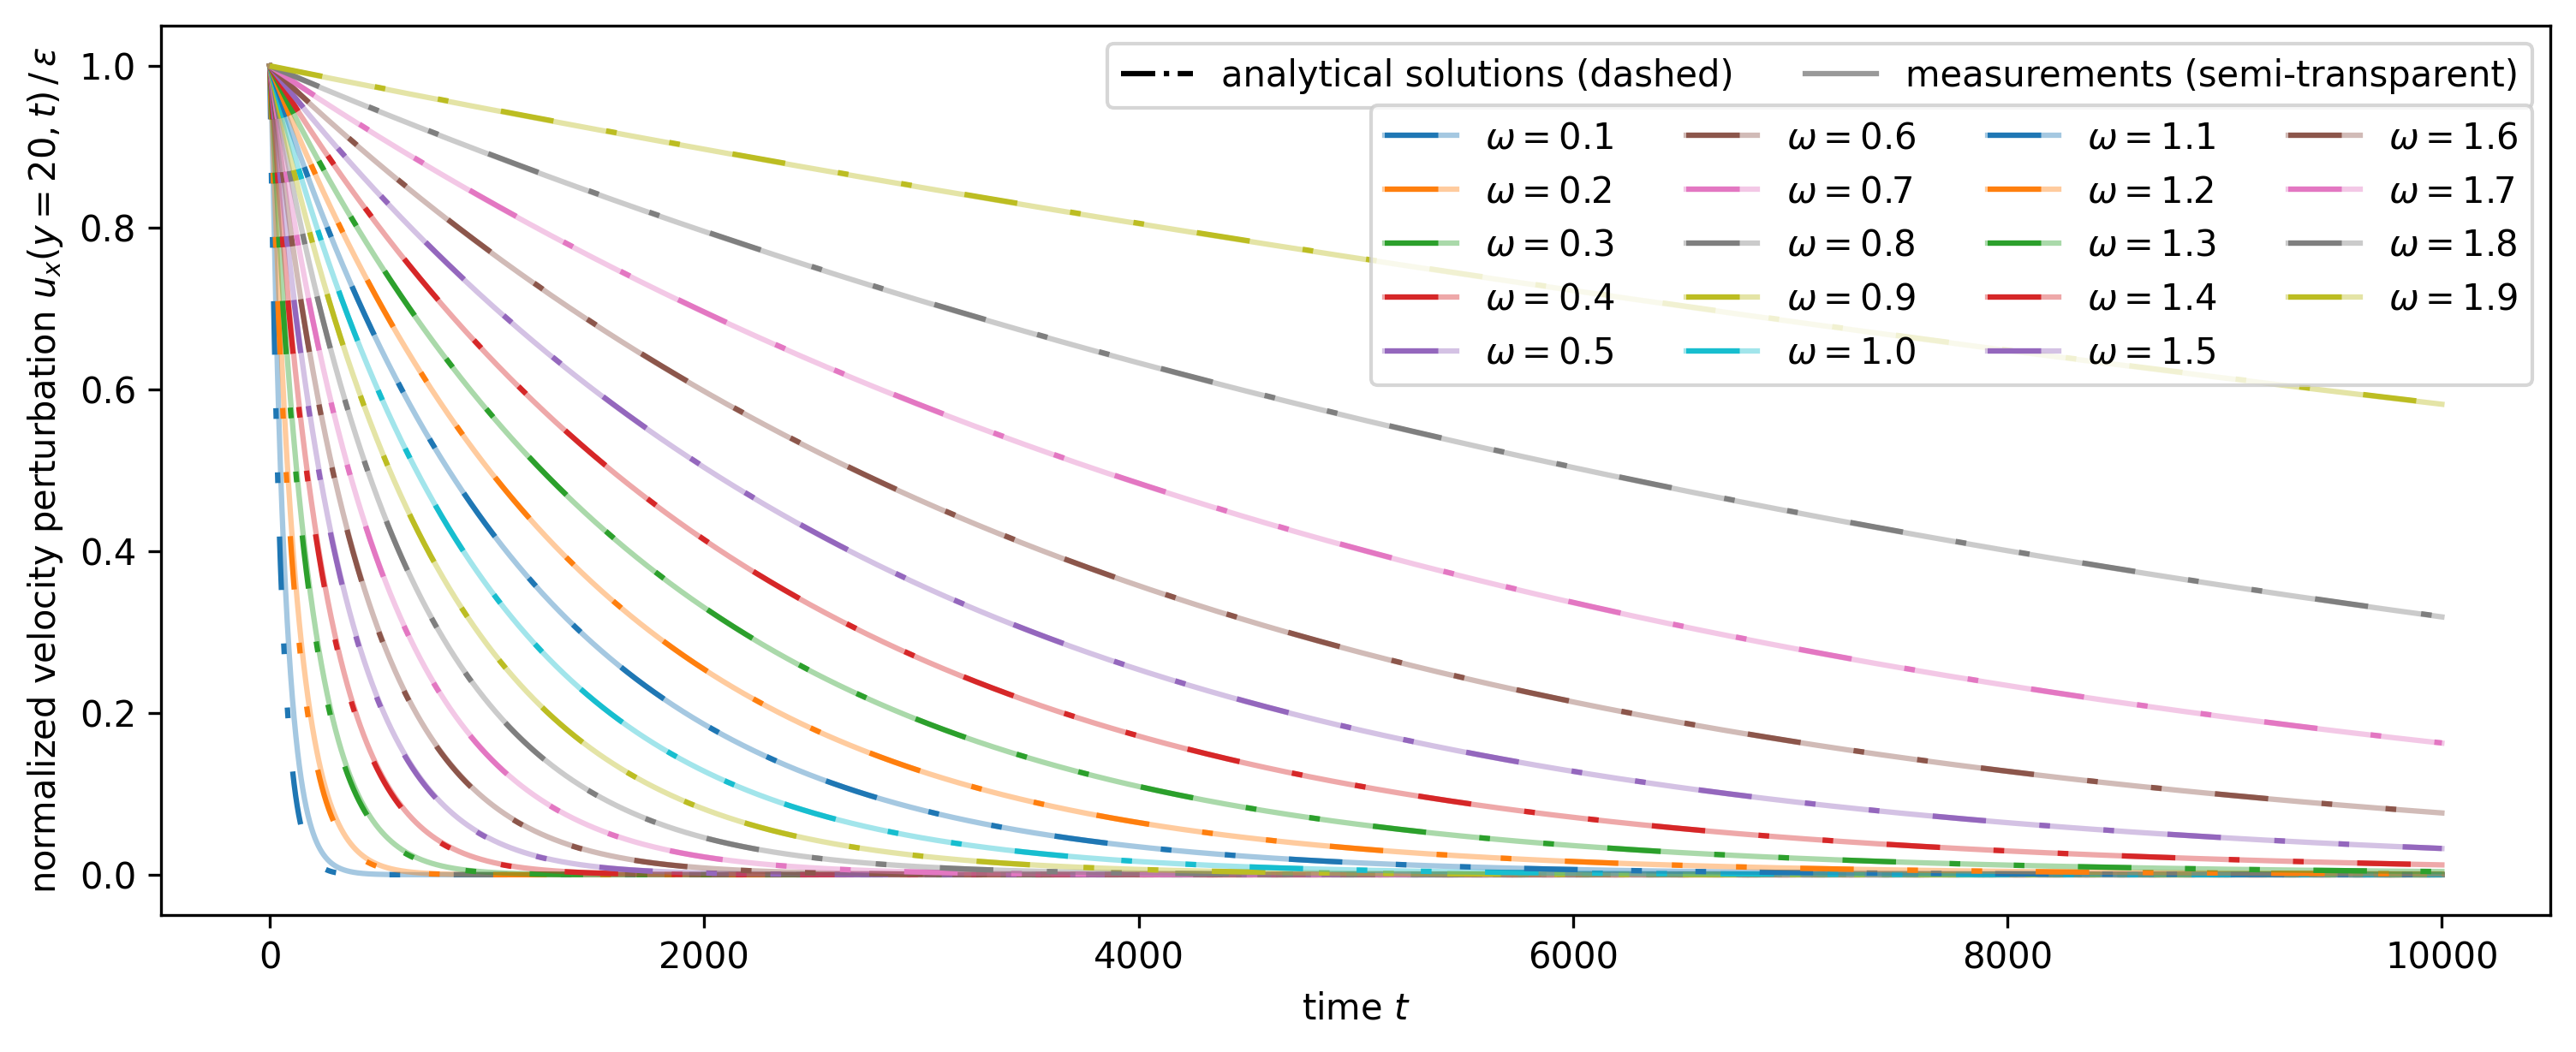
\includegraphics[width=\linewidth]{m3_velocity_decay_different_omegas_normalized.png}
    \caption[Shear Wave Decay: Normalized time evolution of the sinusoidal velocity decay for different relaxation rates $\omega$]{Shear Wave Decay: Normalized time evolution of the sinusoidal velocity decay for different relaxation rates $\omega$. The measured values are given by the velocity at $y=20$ in $x$-direction for a lattice of size $20\times80$. They are set in relation to the analytical solution given by \cref{eq:swd:analytica-solution}. The simulation was run for $10000$ steps and with an amplitude $\varepsilon=0.1$ for the initial sinusoidal velocity as described by \cref{eq:swd:init-velocity}.}
    \label{fig:swd:velocity:multiple-omega}
\end{figure}

The measured decay can be used to determine the kinematic viscosity $\nu$ of the simulation by fitting the exponential analytical solution in \cref{eq:swd:analytica-solution} to the measured values. In case of the oscillating density decay, only the peaks get fitted. \cref{fig:swd:viscosity} shows the results of this for different relaxation rates $\omega$ and compares it to the expected analytical prediction. This expected viscosity is determined through a direct relation to the relaxation rate $\omega$ as given in \cref{eq:omega-to-viscosity}, where $c_s=\sqrt{\frac{1}{3}}$ is the speed of sound in lattice dimensions:
\begin{equation}
    \nu = c_s^2 \left(\frac{1}{\omega} - \frac{1}{2}\right)
    \label{eq:omega-to-viscosity}
\end{equation}

\begin{figure}[ht!]
    \begin{subfigure}{0.5\linewidth}
        \centering
        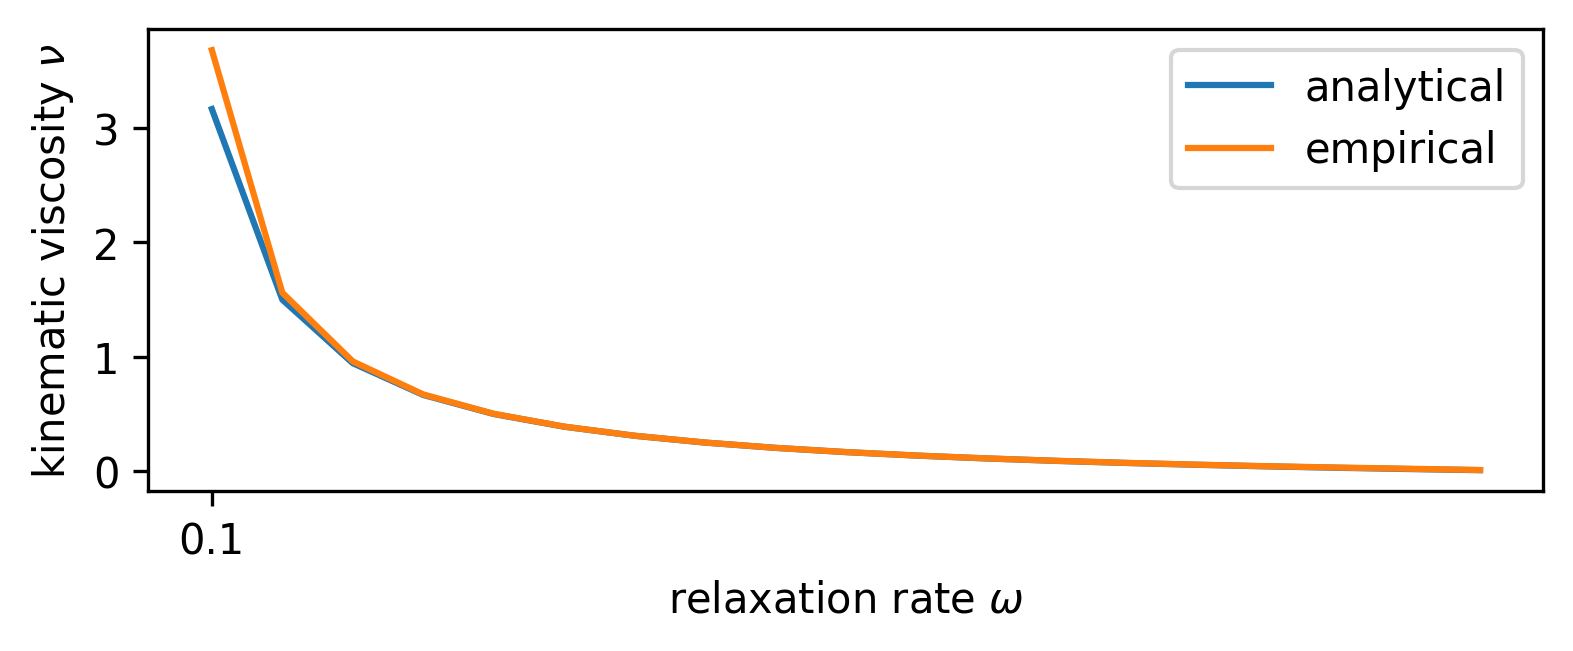
\includegraphics[width=\linewidth]{m3_density_viscosity.png}
        \caption{Sinusoidal density decay}
        \label{fig:swd:density:viscosity}
    \end{subfigure}%
    \begin{subfigure}{0.5\linewidth}
        \centering
        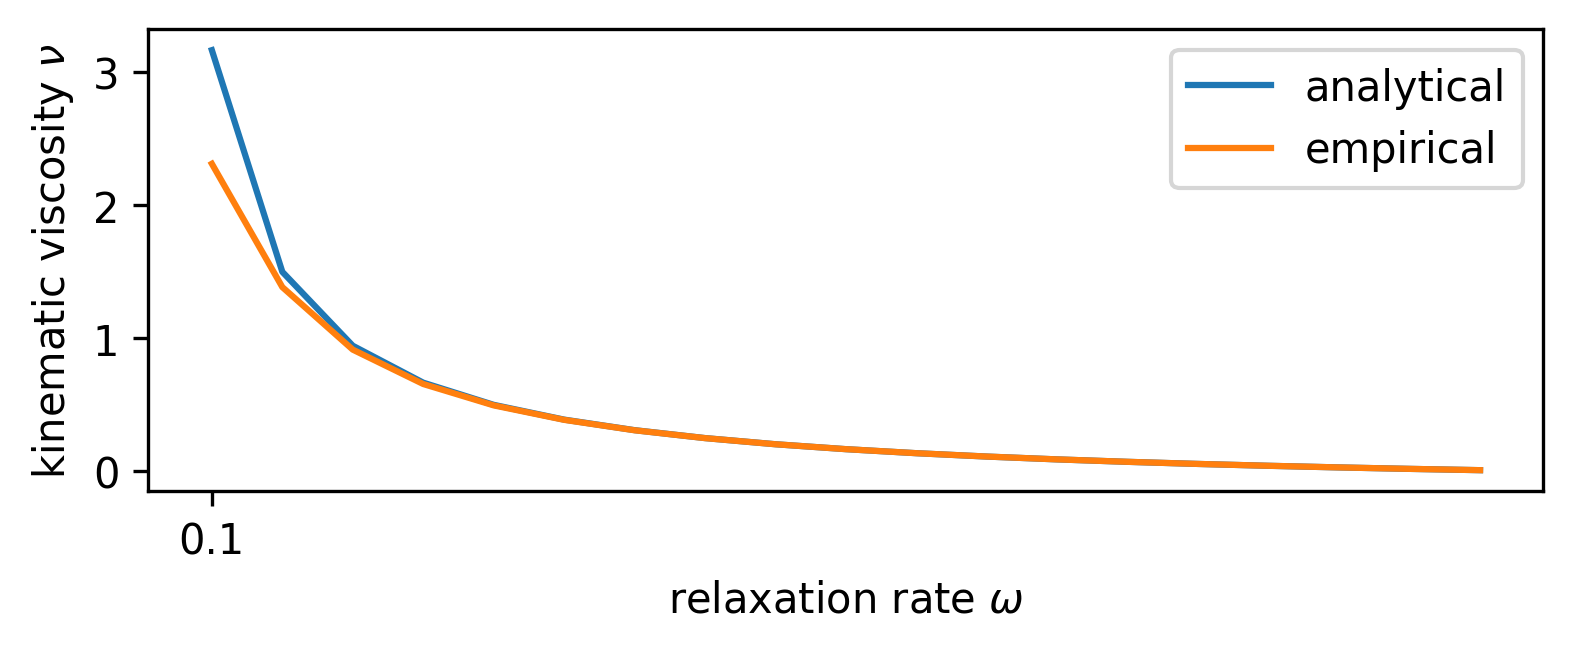
\includegraphics[width=\linewidth]{m3_velocity_viscosity.png}
        \caption{Sinusoidal velocity decay}
        \label{fig:swd:velocity:viscosity}
    \end{subfigure}
    \caption[Shear Wave Decay: Scaling of the kinematic viscosity $\nu$ with respect to the relaxation rate $\omega$]{Shear Wave Decay: Scaling of the kinematic viscosity $\nu$ with respect to the relaxation rate $\omega$. The analytical solution is given by \cref{eq:omega-to-viscosity}. The empirical results are obtained by fitting (a) $||u_x||$ or (b) $||\rho-\rho_0||$ to the exponential given in \cref{eq:swd:analytica-solution}. The parameters for (a) and (b) are the same as in \cref{fig:swd:density:multiple-omega,fig:swd:velocity:multiple-omega} respectively.}
    \label{fig:swd:viscosity}
\end{figure}

Overall, the shear wave decay yielded the expected results as shown in \cref{fig:swd:sines,fig:swd:density:decay,fig:swd:velocity:multiple-omega,fig:swd:viscosity}. This validates the implementation of the streaming and collision operation. However, it also showed that $\omega$ values close to 0 or 2 should be avoided. A relaxation rate close to 0 gives inaccurate viscosity values as seen in \cref{fig:swd:viscosity}, while relaxation rates close to 2 can lead to an instable simulation as indicated by the large derivation from the analytical solution for $\omega=1.9$ in \cref{fig:swd:density:multiple-omega}. Even though in the case of the shear wave decay, $\omega=1$ remained stable for more than 10000 steps and eventually also converged to the analytical solution, this may not be the case for other less artificial scenarios.

\subsection{Couette Flow}

Couette flow is the flow in a viscous fluid between two boundaries of which one is rigid and one is moving with velocity $U_w$. In the considered case the rigid wall is at the bottom boundary, the moving wall is at the top ($y=0$) and moves to the right as illustrated in \cref{fig:concept:couette}. One the inlet (left) and outlet (right), \glsentrylongpl{PBC} are applied.

The moving wall induces a flow that propagates through the fluid due to the viscosity. In the steady state, a linear velocity in $x-direction$ should be obtained for which an analytical solution is given by:
\begin{equation}
    u_x(y) = \left(1-\frac{y}{L_y}\right) U_w
    \label{eq:couette:analytical-solution}
\end{equation}

\cref{fig:couette} shows the results of the Couette flow experiment and that both the velocity field and profile evolve as expected. In the beginning the velocity profile has the highest values at the moving wall. Over time, the flow propagates to the bottom and eventually converges to the analytical solution.

Therefore, the obtained results validate the implementation of the moving wall boundary condition.

\begin{figure}[ht!]
    \begin{subfigure}{0.5\linewidth}
        \centering
        \begin{tikzpicture}[font=\footnotesize, x=9mm, y=8mm]
            \draw[line width=1.2pt] (0,0) -- node[midway, below] {rigid wall} +(6,0);
            \draw[line width=1.2pt, color=red, -Latex] (0,3) -- node[midway, above] {moving wall} +(6,0) node[pos=1, above] {$U_w$};
            \draw[dashed] (2,3) -- (2,0);
            \draw[color=blue] (4,3) -- (2,0);
            \foreach \i in {1,...,11}
                \draw[-Latex, color=blue] (2,{0.25*\i}) -- +({0.25*2/3*\i},0);
            \node[color=blue, anchor=west, align=center] at (3.25,1.5) {analytical\\solution};
        \end{tikzpicture}
        \caption{Couette flow}
        \label{fig:concept:couette}
    \end{subfigure}%
    \begin{subfigure}{0.5\linewidth}
        \centering
        \begin{tikzpicture}[font=\footnotesize, x=9mm, y=8mm]
            \draw[line width=1.2pt] (0,0) -- node[midway, below] {rigid wall} +(6,0);
            \draw[line width=1.2pt] (0,3) -- node[midway, above] {rigid wall} +(6,0);
            \draw[dashed] (1.5,3) -- (1.5,0);
            \draw[color=blue, variable=\y, domain=-1.5:1.5, smooth]  plot ({-\y*\y+3.75}, {\y+1.5});
            \foreach \i in {1,...,11}
                \draw[-Latex, color=blue] (1.5,{0.25*\i}) -- +({2.25-(1.5-\i*0.25)*(1.5-\i*0.25)},0);
            \node[color=blue, anchor=south west, align=center] at (3.75,1.5) {analytical\\solution};
            \draw[-Latex] (0,1) -- +(1,0) node[midway, above] {inlet} node[midway, below] {$p + \Delta p$};
            \draw[-Latex] (5,1) -- +(1,0) node[midway, above] {outlet} node[midway, below] {$p$};
        \end{tikzpicture}
        \caption{Poiseuille flow}
        \label{fig:concept:poiseuille}
    \end{subfigure}
    \caption{Conceptual visualization of the Couette and Poiseuille flows.}
    \label{fig:concept:couette-and-poiseuille}
\end{figure}

\begin{figure}[ht!]
    \begin{subfigure}{\linewidth}
        \centering
        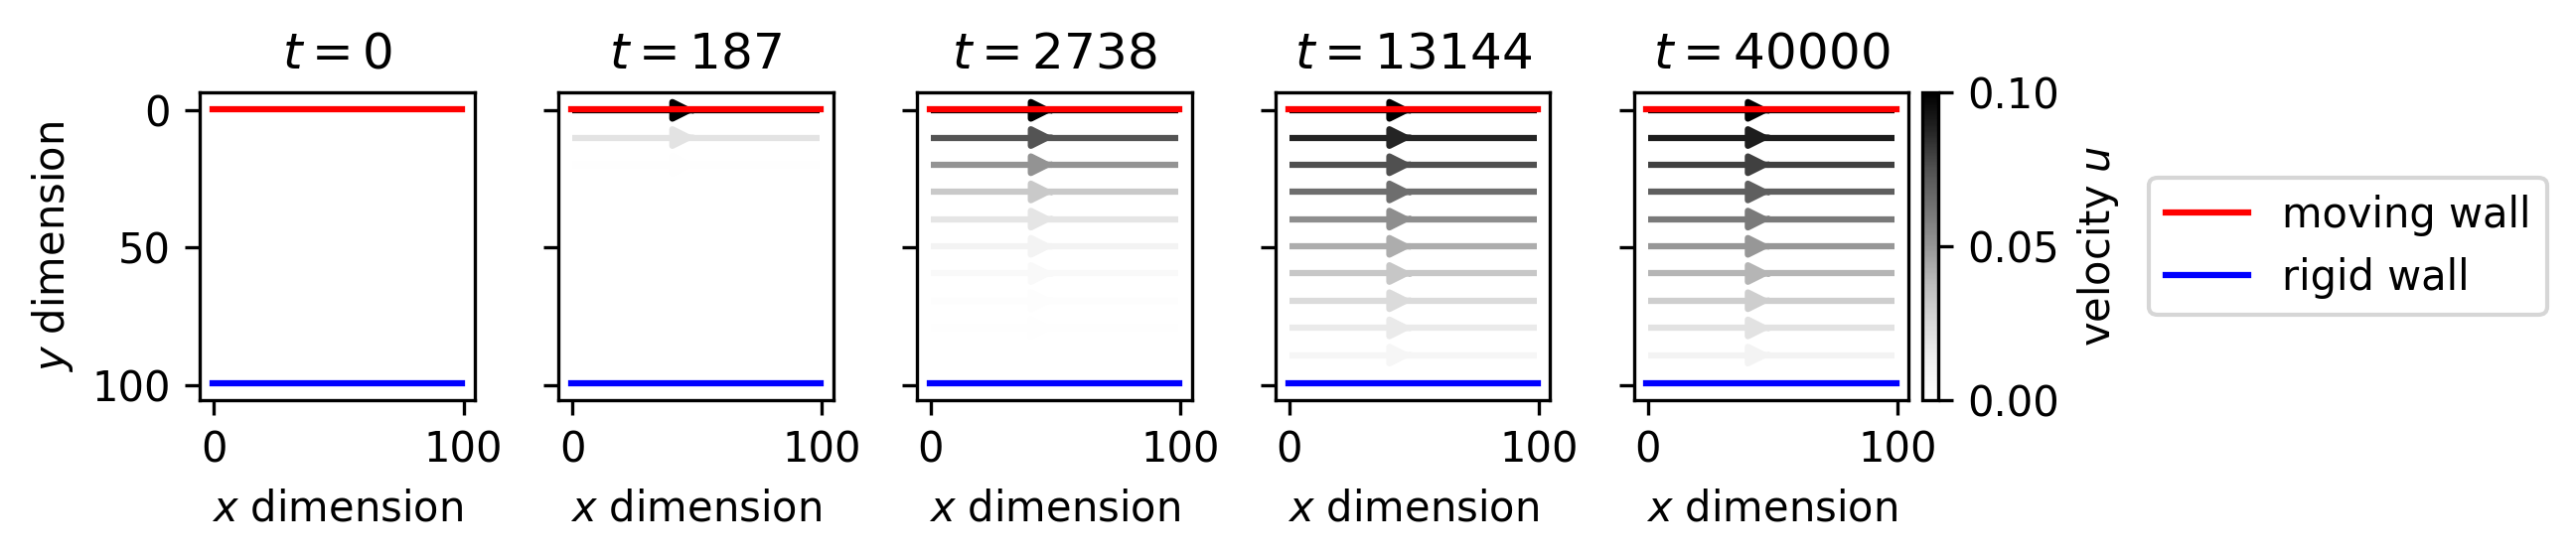
\includegraphics[width=\linewidth]{m4_velocity_flow_field_evolution.png}
        \caption{Velocity field}
        \label{fig:couette:flow-field}
    \end{subfigure}

    \begin{subfigure}{\linewidth}
        \centering
        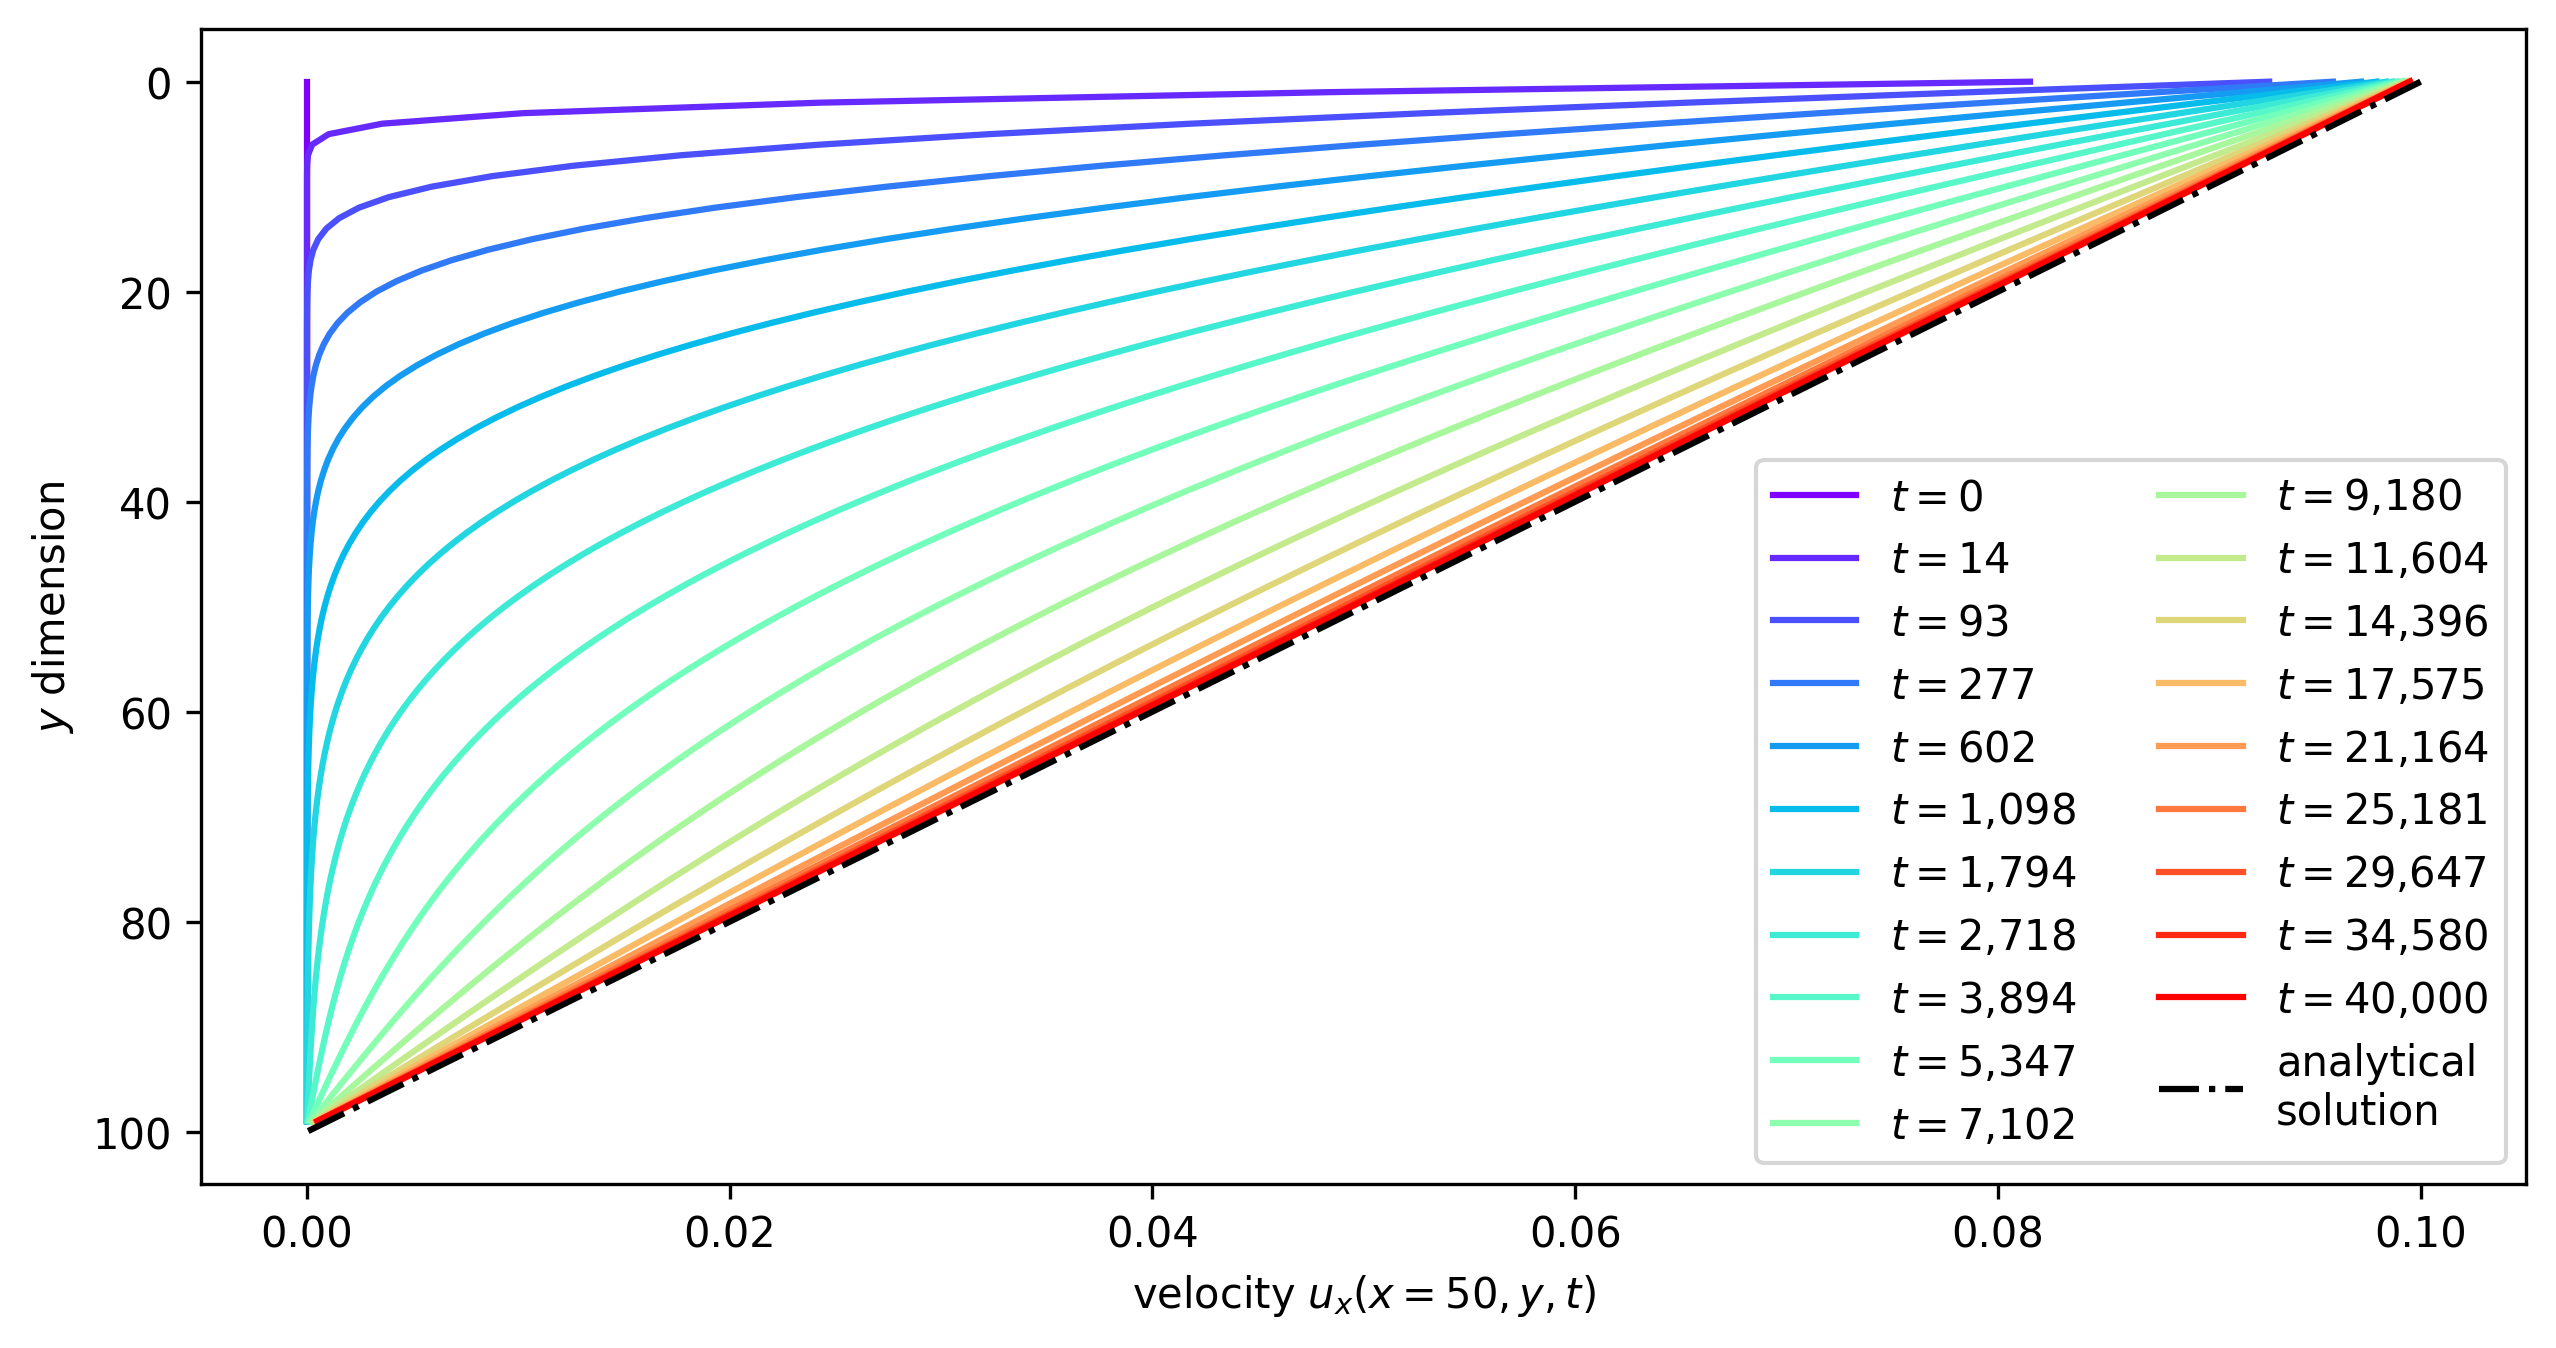
\includegraphics[width=0.8\linewidth]{m4_velocity_profile_evolution.png}
        \caption{Velocity profile}
        \label{fig:couette:profile}
    \end{subfigure}
    \caption[Couette Flow]{Couette Flow. Evolution of the velocity field and profile according to the Couette flow experiment. The results where obtained with a $100\times100$ lattice, an initial density $\rho(t=0)=1$, an initial velocity $u(t=0)=0$, a relaxation rate $\omega=1.0$, a wall velocity $U_w=0.1$ and $40000$ simulation steps.}
    \label{fig:couette}
\end{figure}

\subsection{Poiseuille Flow}

Poiseuille flow is the flow between two rigid walls as illustrated in \cref{fig:concept:poiseuille}. The flow is induced by a constant pressure gradient $\frac{dp}{dx}$ between the inlet and outlet. In the considered setting, the rigid walls are at the top and bottom boundaries, inlet (left) and outlet (right) are implemented using \glspl{PBC} with a pressure gradient. Instead of a pressure variation $\Delta p$ between inlet and outlet, a density variation $\Delta \rho$ is applied, since pressure is directly related to density through the ideal gas equation of state:
\begin{equation}
    p = c_s^2 \rho
    \label{eq:pressure-density-relation}
\end{equation}
In the steady state, a parabolic velocity profile should be obtained, for which the analytical solution is given by:
\begin{equation}
    u_x(y) = - \frac{1}{2\rho\nu} \frac{dp}{dx} y (Y-y)
    \label{eq:poiseuille:analytical-solution}
\end{equation}

\cref{fig:poiseuille} presents the results obtained from the Poiseuille flow experiment. It shows how the velocity profile over time converges to the analytical solution and that a linear density gradient is obtained between the inlet and outlet. These results validate the correct implementation of the \glspl{PBC} with pressure gradient.

\begin{figure}[ht!]
    \begin{subfigure}{0.53\linewidth}
        \centering
        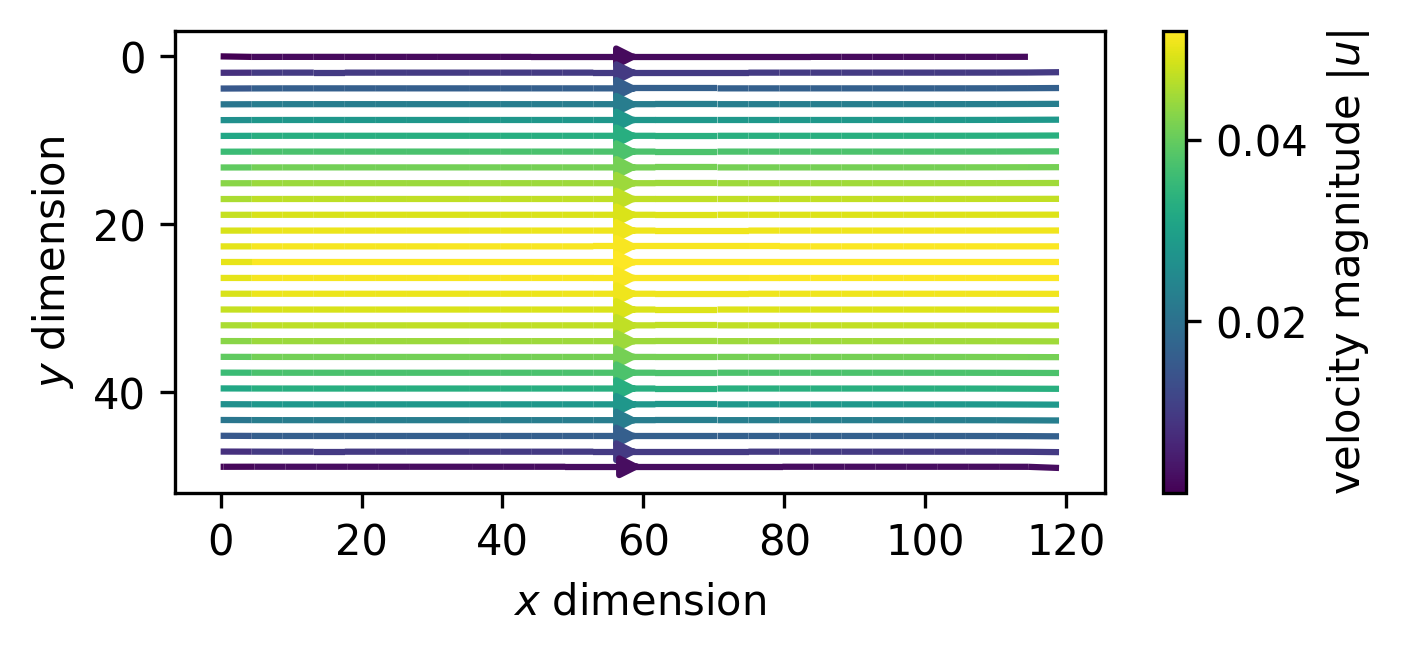
\includegraphics[width=\linewidth]{m5_velocity_field.png}
        \caption{Velocity field in the steady state}
        \label{fig:poiseuille:flow-field}
    \end{subfigure}%
    \begin{subfigure}{0.47\linewidth}
        \centering
        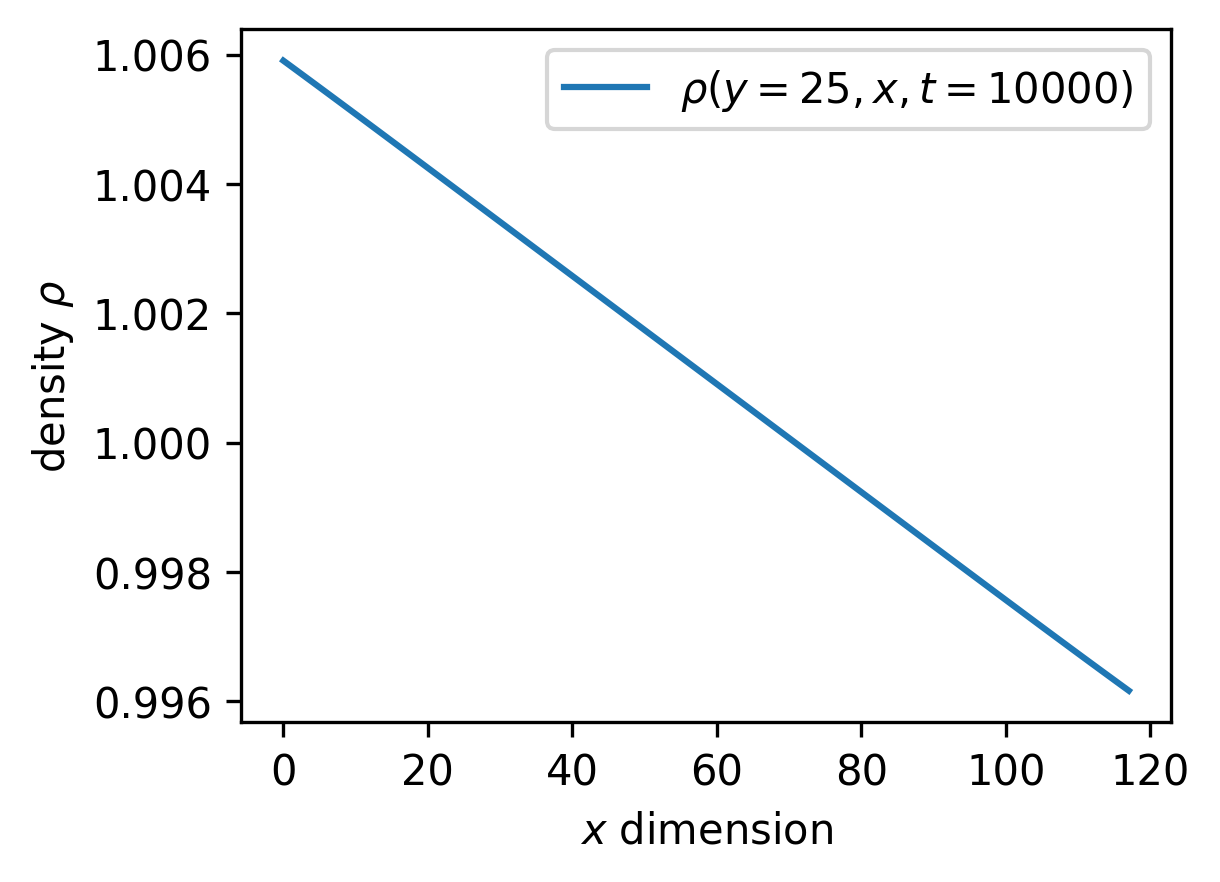
\includegraphics[width=\linewidth]{m5_density_along_centerline.png}
        \caption{Density along centerline}
        \label{fig:poiseuille:density-centerline}
    \end{subfigure}

    \begin{subfigure}{\linewidth}
        \centering
        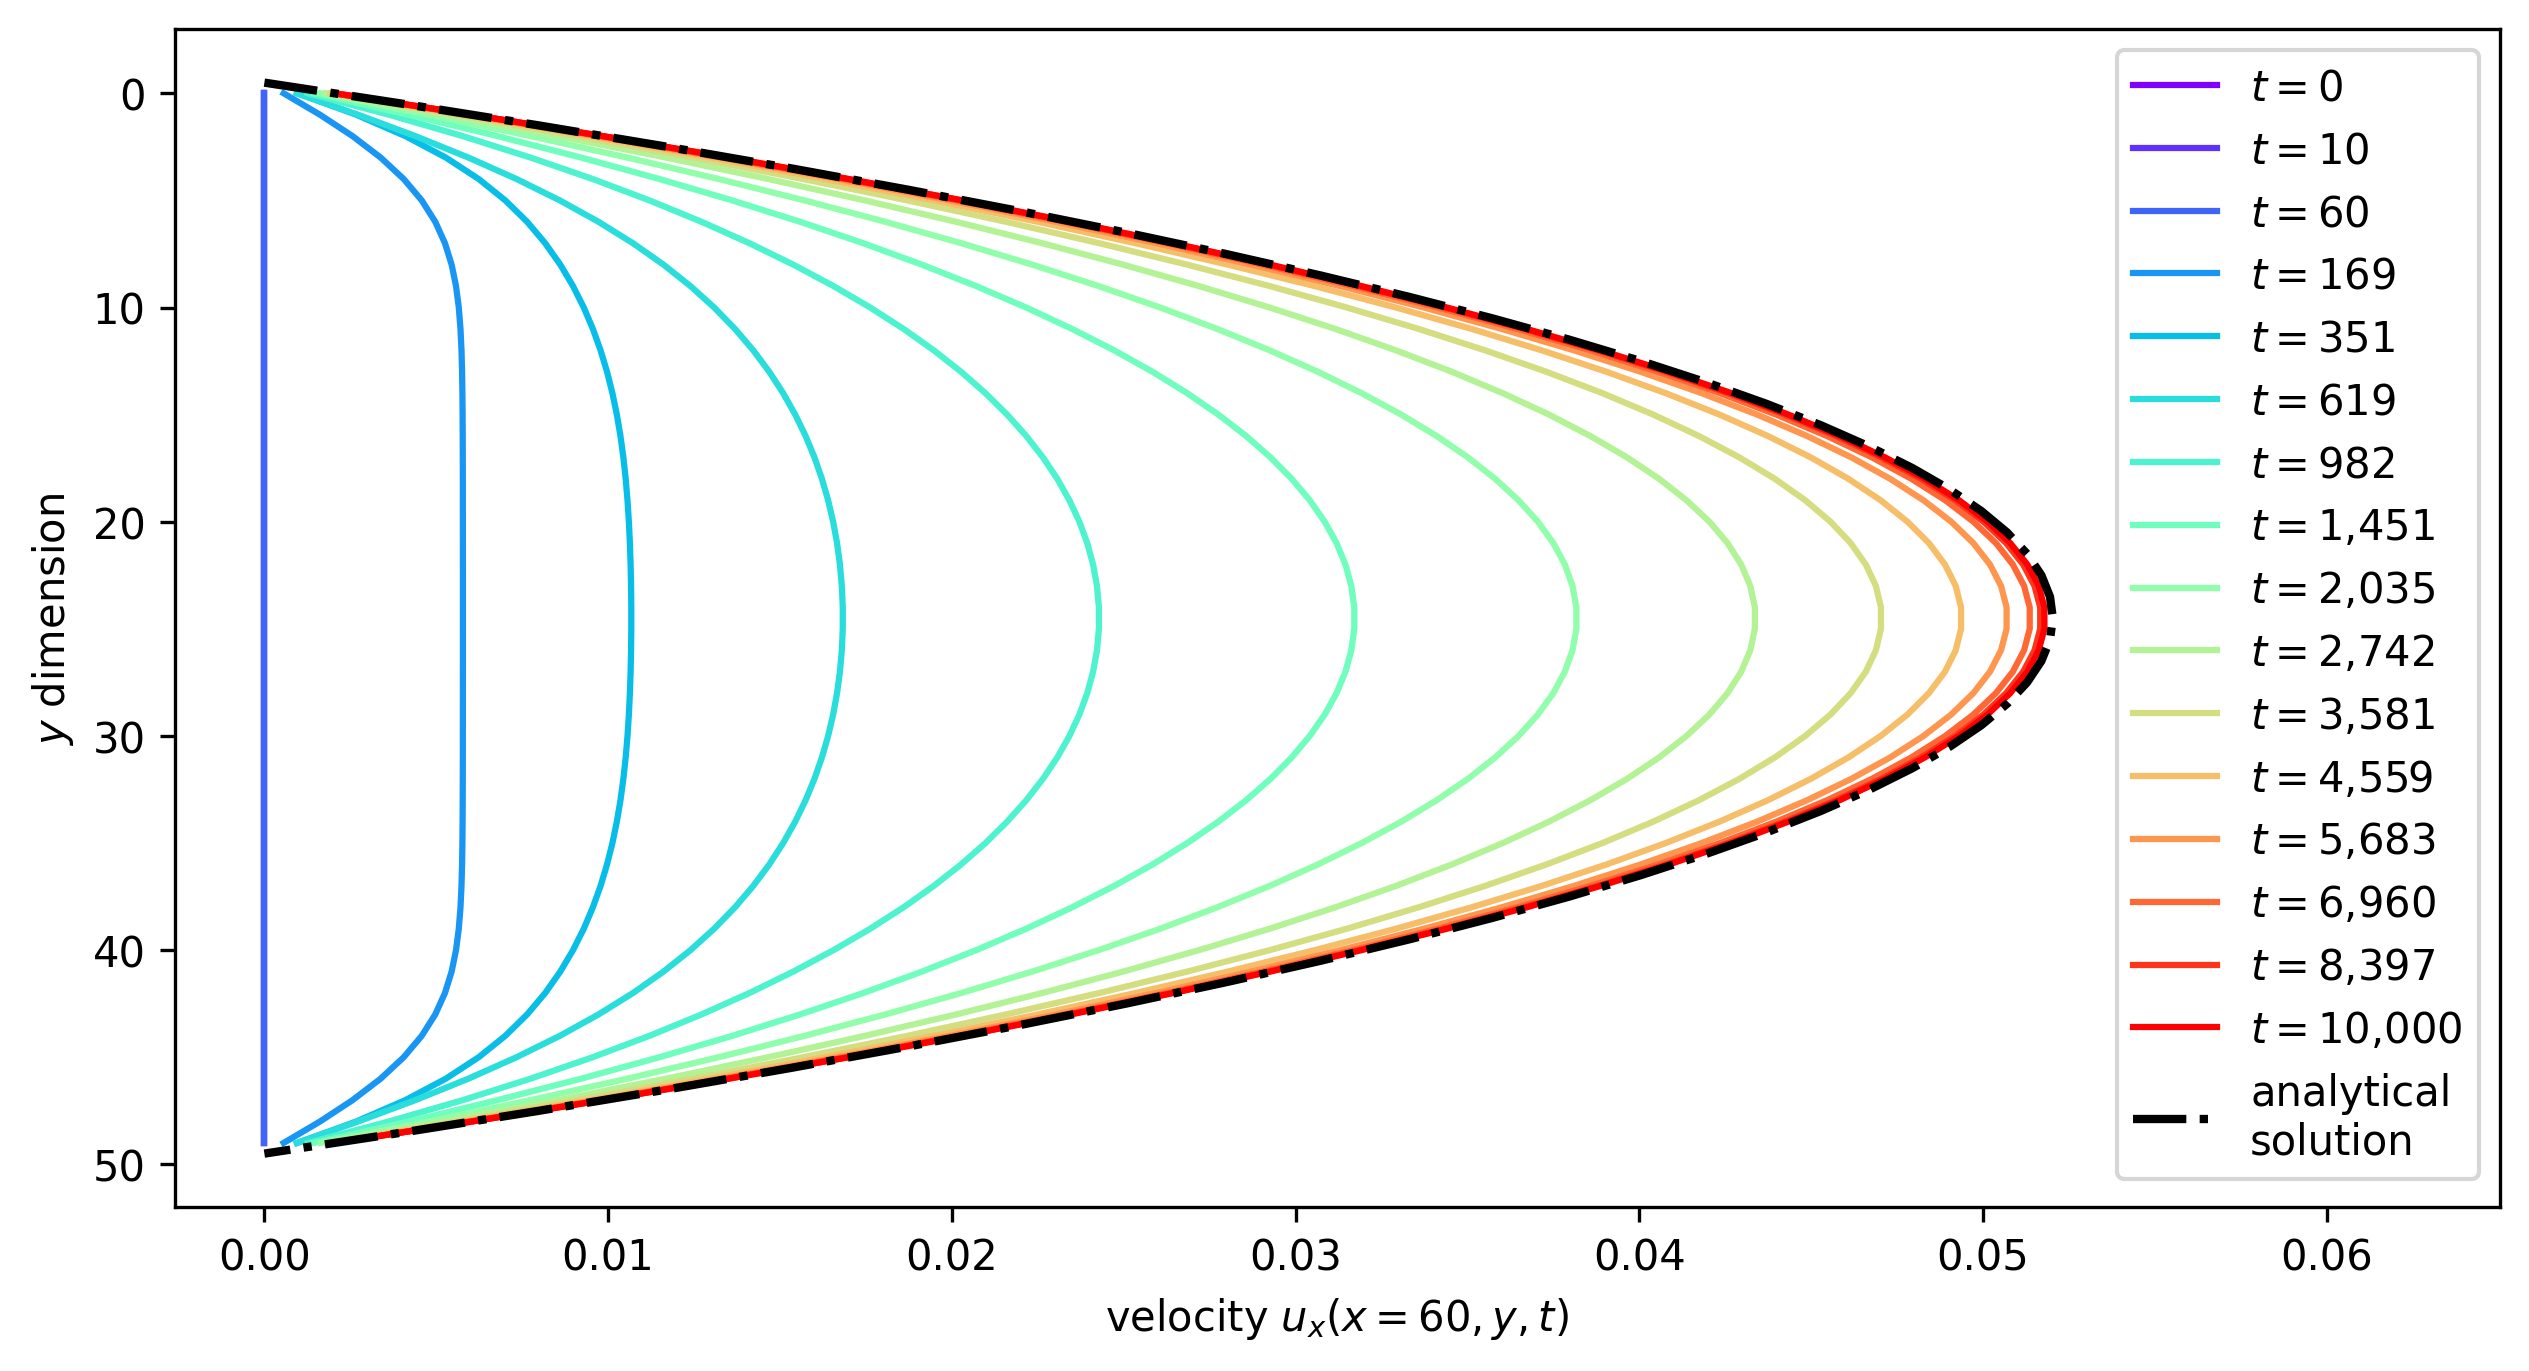
\includegraphics[width=0.8\linewidth]{m5_velocity_profile_evolution.png}
        \caption{Evolution of the velocity profile}
        \label{fig:poiseuille:profile}
    \end{subfigure}
    \caption[Poiseuille Flow]{Poiseuille Flow. Evolution of the velocity field and profile as well as the resulting density gradient according to the Poiseuille flow experiment. The results were obtained with a $120\times50$ lattice, an initial density $\rho(t=0)=1$, an initial velocity $u(t=0)=0$, a relaxation rate $\omega=1.0$, a density gradient from $\rho_{in}=1.005$ to $\rho_{out}=0.995$ and $10000$ simulation steps.}
    \label{fig:poiseuille}
\end{figure}

\subsection{Lid-Driven Cavity}

The lid-driven cavity is a well-known benchmark for fluid simulations. It consists of a square cavity with three rigid and one moving wall, the sliding lid. In the considered setting, the lid is located at the top boundary and moves to the right with velocity $U_w$. The sliding lid induces turbulences in the cavity, which are characterized by the Reynolds number $Re$, a dimensionless number which expresses the ratio between the inertial terms and the viscous ones and helps to predict flow patterns:
\begin{equation}
    \label{eq:reynolds-number}
    Re = \frac{Lu}{\nu}
\end{equation}
In this equation $L$ is a characteristic length, which in case of a square cavity is simply the domain size $L=L_x=L_y$, and $u$ corresponds to the wall velocity $U_w$ and.

\cref{fig:lid:streamplots} shows the steady-state velocity fields of the lid-driven cavity experiment for different Reynolds numbers and viscosity values. It demonstrates, that for the same Reynolds number, the resulting flow is almost the same, despite differences in the viscosity. For example the eddy in the bottom-left corner gets more distinct with higher Reynolds numbers. A video of the time evolution of the velocity field is available in the code repository\footnote{\therepository}.

\begin{figure}[htp]
    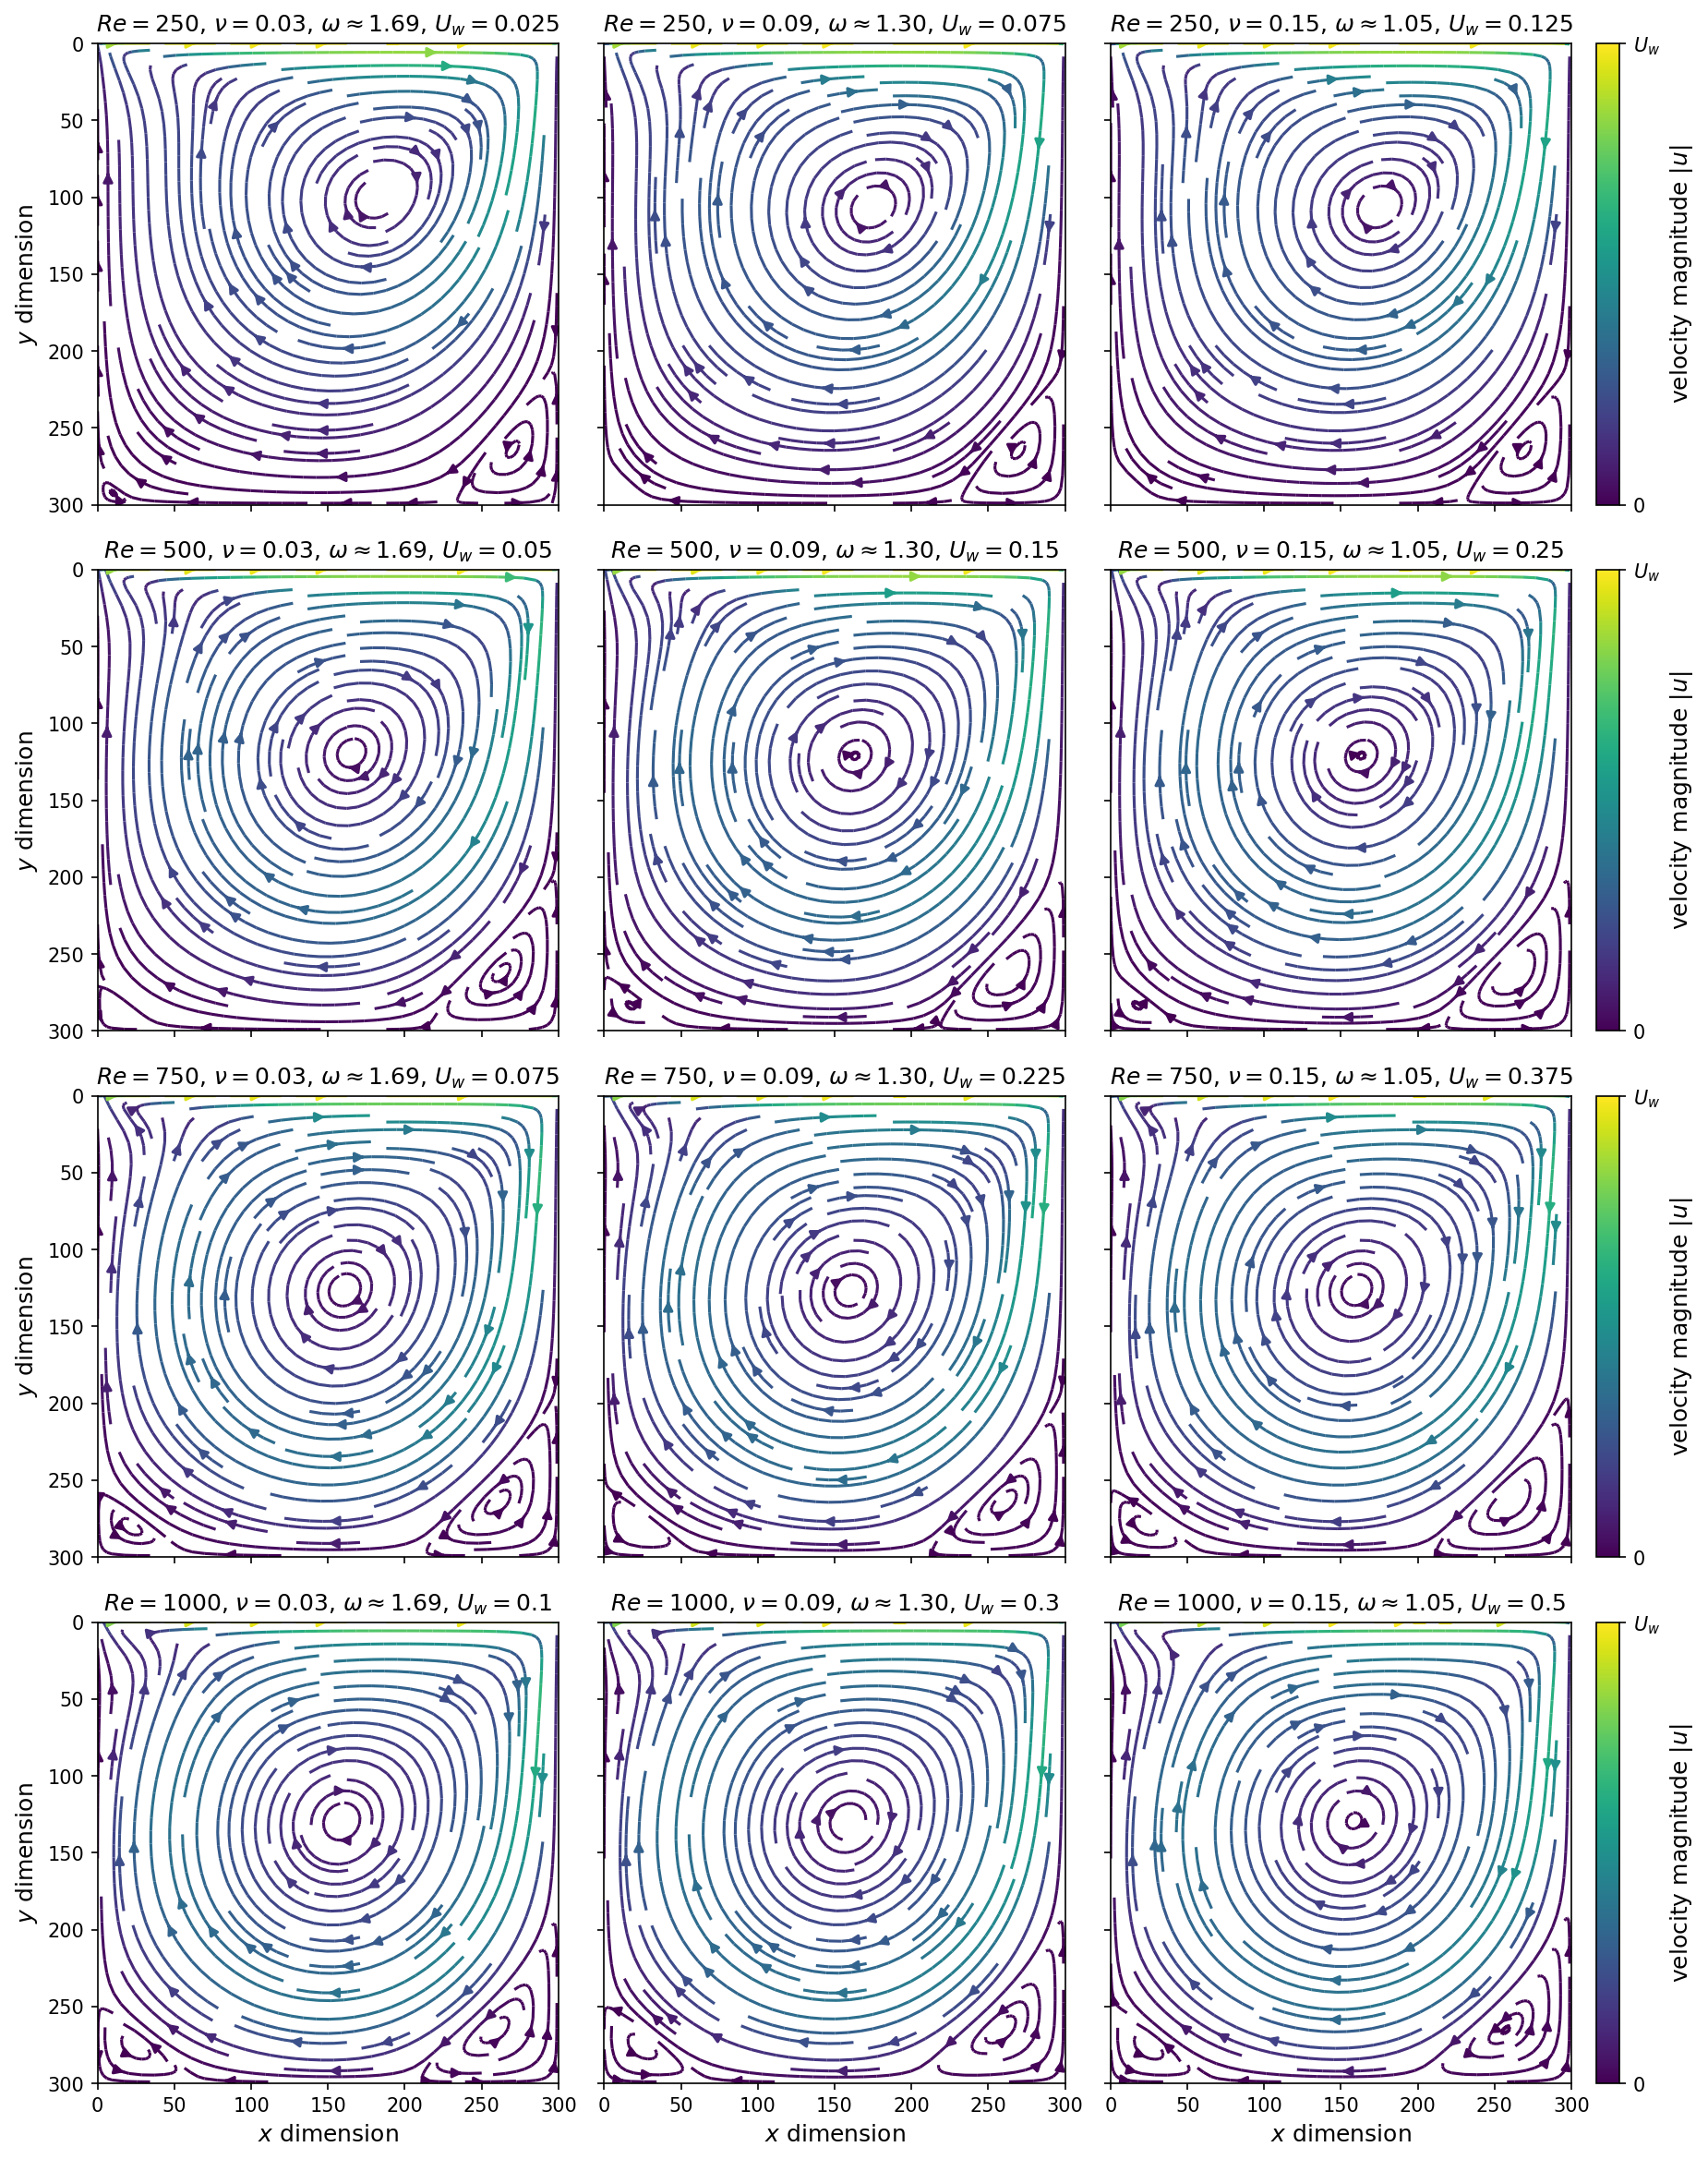
\includegraphics[width=\linewidth]{m6_streamplots.png}
    \caption[Lid-Driven Cavity: Streamline plots for different Reynolds numbers]{Lid-Driven Cavity: Streamline plots for different Reynolds numbers. Each simulation was run with a $300\times300$ lattice and a given set of combinations of different Reynolds numbers $Re$ and viscosity values $\nu$ for $100000$ steps. Density and velocity were initialized with $\rho(t=0)=1$ and $u(t=0)=0$. The relaxation rate $\omega$ and wall velocity $U_w$ are deduced values, following \cref{eq:omega-to-viscosity,eq:reynolds-number}.}
    \label{fig:lid:streamplots}
\end{figure}

Note that the plots in \cref{fig:lid:streamplots} were computed without parallelization. For a couple of cases, the resulting velocity fields of both the serial and the parallel implementation were compared. It could be observed, that both were identical. Therefore, it can be concluded, that the parallelization is implemented correctly.

\subsection{Scaling}

In order to test, how good the parallel implementation scales, the lid-driven cavity experiment was run multiple for different lattice sizes and different number of MPI processes. The scaling test were run on the bwUniCluster 2.0\footnote{\href{https://wiki.bwhpc.de/e/Category:BwUniCluster\_2.0}{https://wiki.bwhpc.de/e/Category:BwUniCluster\_2.0}}. To compare the result, the number of \glsentryfull{MLUPS} is used as measure. It is calculated from the lattice dimensions $L_x \times L_y$, the total number of simulation steps $N_{steps}$ and the elapsed time $T$ as given by the following equation:

\begin{equation}
    \label{eq:mlups}
    \text{MLUPS} = \frac{L_x \cdot L_y \cdot N_{steps}}{10^6 \cdot T}
\end{equation}

The results are displayed in \cref{fig:lid:scaling}. It can be observed, that for a few processes it scales linearly. This diminishes as the number of processes grows and therefore the size of each subdomain shrinks. An intuition for the observed behavior is given by Amdahl's Law \cite{amdahl}. The non-optimal speedup is caused by the necessary synchronization between processes imposed by the communication step. Decreasing of the speedup starts when the perimeter-to-area ratio grows large enough, roughly $>0.1$, and hence the additional cost of the communication eventually outweighs the benefit gained by the parallelization.

\begin{figure}[ht!]
    \centering
    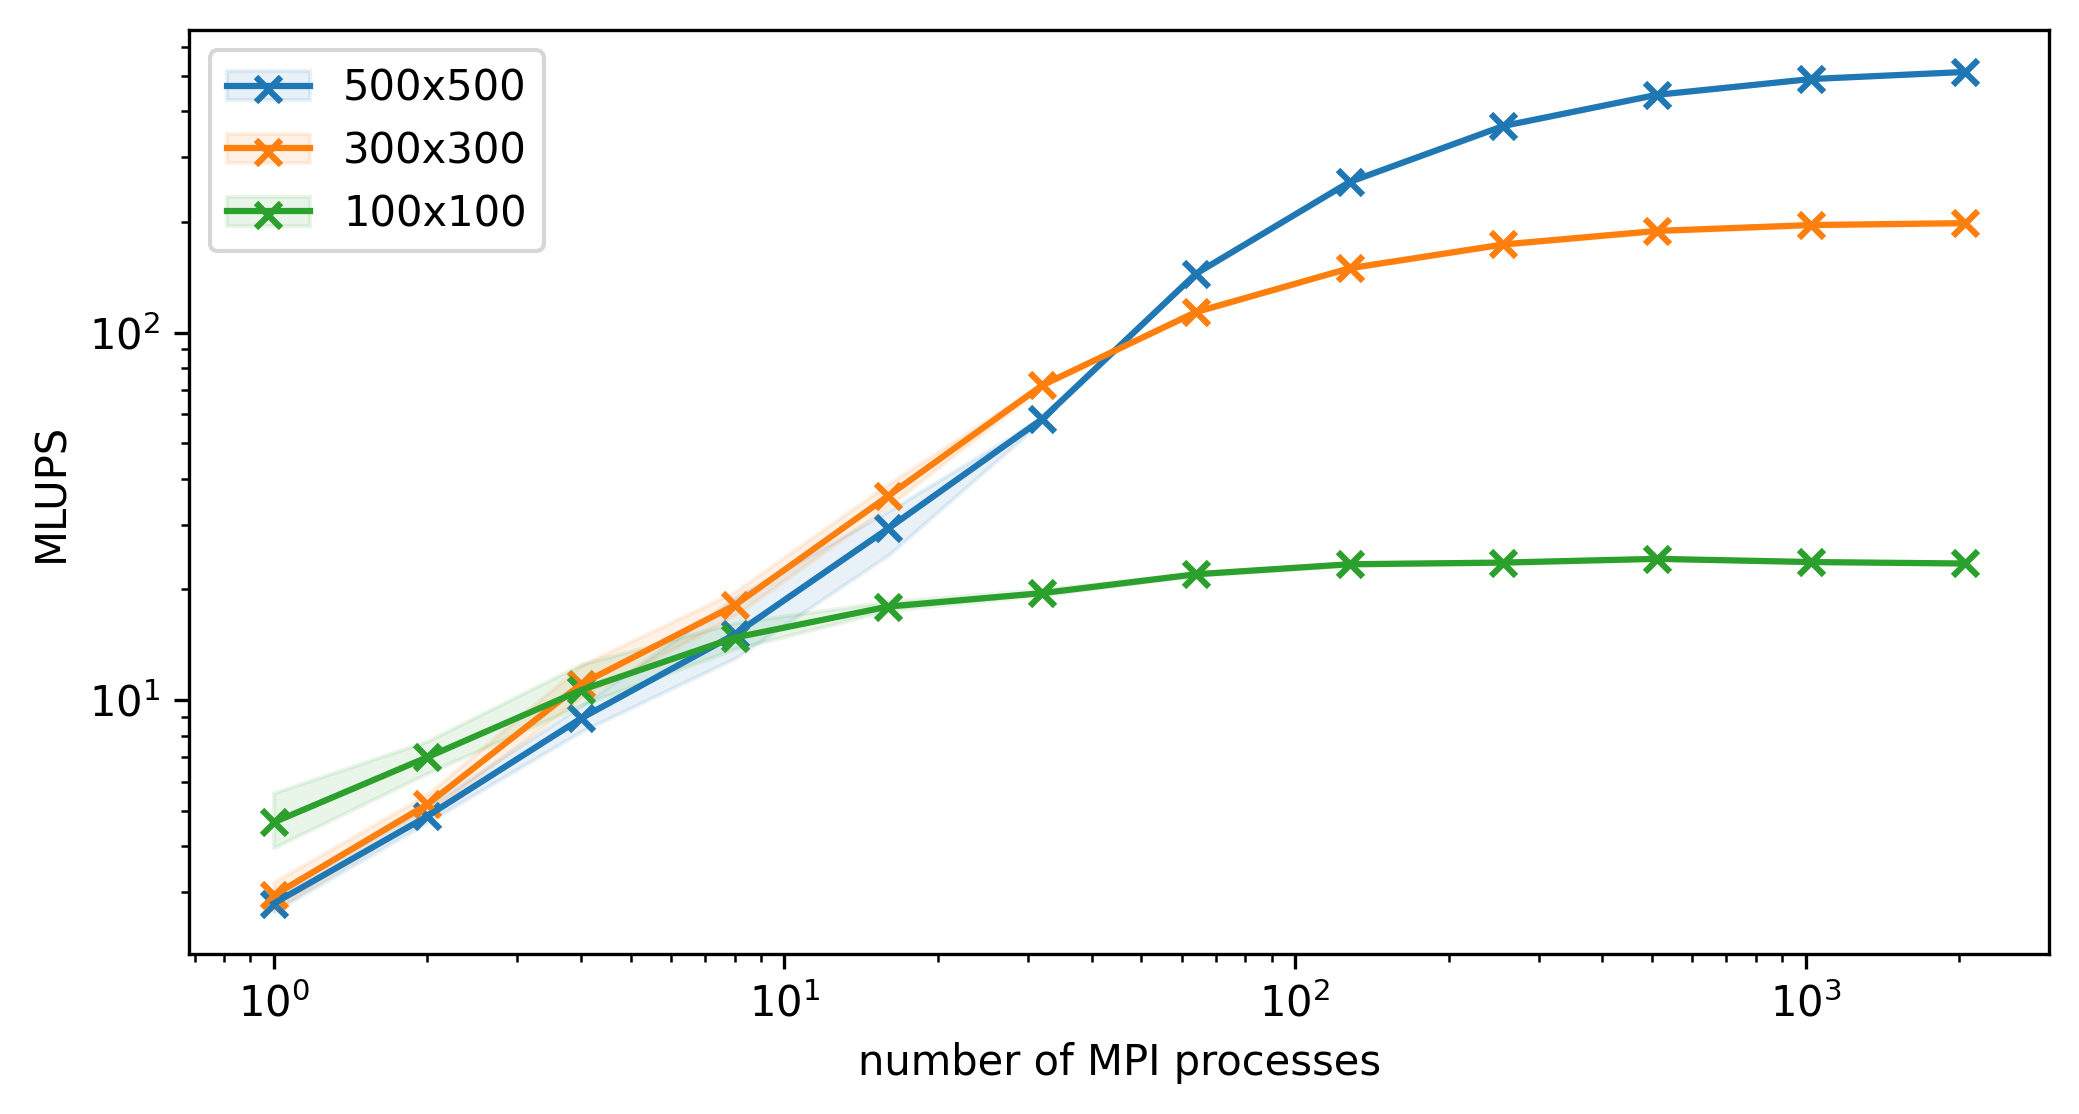
\includegraphics[width=\linewidth]{m7_mlups.png}
    \caption[Scaling behavior of the lid-driven cavity simulation]{Scaling behavior of the lid-driven cavity simulation. The number of MPI processes was chosen to be from the set $\{2^x~|~0 \le x \le 12,~ x \in \mathbb{N}\}$. Each test case was run three times. The crosses represent the mean value for each test case, while the light regions around the curve indicate the minimum and maximum values. All simulations were run with a relaxation rate $\omega=1.7$, a wall velocity $U_w=0.1$ and a total of 100000 steps. The \gls{MLUPS} number is calculated from the measured elapsed time using \cref{eq:mlups}.}
    \label{fig:lid:scaling}
\end{figure}

    \section{Conclusions}

This report demonstrated a parallel implementation of the \glsentryfull{LBM} for simulating fluid dynamics. Implementation was done in the Python programming language and the NumPy library for efficient numerical calculations. For the parallelization, the \glsentryfull{MPI} and the respective Python bindings mpi4py were employed.

The implementation was validated using several experiments including shear wave decay, Couette flow, Poiseuille flow and lid-driven cavity. The obtained results coincide with the expected analytical solutions. Therefore, it can be assumed that the implementation is correct.

Furthermore, the scaling behavior of the parallelized implementation was tested by simulating the lid-driven cavity with different number of processes on the bwUniCluster. This showed, that the \gls{LBM} has good scaling behavior. While the subdomain size handled by each MPI process is large enough, it scales linearly. Once the cost imposed by the necessary communication between neighboring subdomains outweighs the benefit gained by the parallelization, the speedup decreases and eventually stagnates.

\section*{Acknowledgements}

The author acknowledges support by the state of Baden-Württemberg through bwHPC.


    % bibliography
    \pdfbookmark{References}{bib}
	% TODO: remove \nocite
	\nocite{*}
    \printbibliography[title=References]

\end{document}
